\chapter{Bayesian Inference of Plasma Diffusion Parameters}\label{chapter:bayes_diff_chapter}

{\small
  We present a novel method which combines sparse irregular observations of a field with its 
  governing physical dynamics, for performing Bayesian inference over latent system parameters. Our 
  method uses a basis function approach coupled with a least squares support vector machine 
  objective function which weighs differently errors arising due to data fitting and satisfaction 
  of physical constraints. The method is applicable to linear PDE systems, it incorporates physical 
  models into classical least squares techniques for the purpose of data assimilation and 
  uncertainty quantification of latent parameters. We apply this method to the inverse problem of 
  inferring uncertainty estimates of plasma diffusion parameters from sparse observations.
}

\vfill
\sectionlinetwo{DarkGreen}{88}
\vfill

\noindent
    \parbox{\textwidth}{%
        {\small This chapter is based on research which is in preperation for publication.}
    }%


\clearpage


\section{Introduction}

The Earth's radiation belts are the regions of space near the Earth that extend between $2R_E$ 
and $8R_E$ ($R_E = \SI{6372}{\kilo\metre}$, the radius of the Earth), where the terrestrial 
magnetic field traps electrons and ions in complex electromagnetic orbits  \citep{vanAllen}. Since 
their discovery, the belts have been the subject of intensive research due to their complex 
behavior and damaging effects on spacecraft \citep{GUBBY20021723, WellingSatellite, baker2002}.

Radiation belt particles generally execute three types of periodic motion, each with its own 
corresponding adiabatic invariant: gyration around magnetic field lines, bounce along field lines, 
and drift around the Earth. During active times, when conditions change on time scales shorter than 
the periods of motion, adiabaticity can be broken and particle motion can not be simply decomposed 
into the aforementioned components. Particle motion can then be represented diffusively along each 
component via the \emph{Fokker-Planck} equation yielding a useful model of radiation belt dynamics 
\citep{schulz2012particle}.

The third invariant represents the total magnetic flux enclosed within a full particle orbit. It is 
common to use a normalised form of this, the so called Roederer $L^{*}$ \citep{Roederer1970}. It is 
analogous to radial distance from the center of the Earth (in Earth radii) to the equatorial 
crossing point of the bouncing particle. Diffusion in $L^{*}$ alone (the other invariants shall be 
considered conserved) accounts for the capture and inward radial transport of radiation belt 
particles \citep{Roederer1970,JGR:JGR4463}.

One of the main difficulties of using a physics-based model for studying and forecasting energetic 
electrons in the radiation belt is that the parameters that characterise the Fokker-Planck 
equation, namely diffusion tensor and loss term, are not directly observable. Hence, their 
determination is an \emph{inverse problem}, which is generally difficult to solve and can often 
become ill-posed.

In this chapter we propose an inference model which can learn from sparse data while taking into 
account prior knowledge of the system dynamics in the form of a linear partial differential 
equation. The method replaces a standard finite difference solver with a surrogate model which 
tries to fit the observations and the system dynamics. The surrogate is expressed as a basis 
function expansion whose coefficients are computed by formulating a 
\emph{Least Squares Support Vector Machine} (LSSVM) like optimization objective.

In the proceeding sections, we give a short introduction to the radial diffusion equation used in 
magnetospheric physics. After an overview of the parameterizations of the radial diffusion unknowns 
used by the research community, we give a detailed formulation of our proposed method and 
demonstrate how it can be used for performing inference over said diffusion parameters.

\subsection{Plasma Diffusion}

The radial diffusion system is a simplified one dimensional version of the \emph{Fokker-Planck} 
equation. It tracks the time evolution of the \emph{phase space density} of particles, $f$ which is 
governed by \cref{eq:raddiffusion} known as \emph{radial diffusion equation} in the radiation belt 
community \citep{JGRA:JGRA9345}.
%
\begin{equation}\label{eq:raddiffusion}
  \frac{\partial{f}}{\partial{t}} = \ell^2 \frac{\partial}{\partial{\ell}} \left( 
    \frac{\kappa(\ell, t)}{\ell^{2}} \frac{\partial{f}}{\partial{\ell}}
  \right)_{\mathcal{M}, J} - \lambda(\ell, t) f + q(\ell, t)
\end{equation}
%
The \emph{phase space density} $f$ is a function of the spatial coordinate $\ell$ which denotes the 
\emph{Roederer} $L^*$ or \emph{L-shell}, and time $t$. The key quantities in the system above are 
as follows.
%
\begin{enumerate}
\item $f$: The particle density, for a given value of the first and second adiabatic invariants, 
as a function of space $l$ and time $t$.
\item $\kappa(\ell, t)$: A space and time varying diffusion field.
\item $\lambda(\ell, t)$: The particle loss rate, a non-negative quantity which indicates how 
quickly particles are lost from the radiation belts, due to mechanisms other than radial diffusion.
\item $q(\ell, t)$: An optional particle injection rate (or source term). If this term is omitted 
      (i.e. $q(\ell, t) = 0$) then boundary conditions $f(\ell_{min}, t)$ and $f(\ell_{max}, t)$ 
      must be specified to solve \cref{eq:raddiffusion}. 
\end{enumerate}
%
Interested readers can refer to section \S~\ref{sec:plasmadiff} for a more detailed explanation on 
plasma diffusion, adiabatic invariants and plasma motion in the Earth's radiation belts. 

\subsubsection*{Diffusion Parameters}

To solve the radial diffusion system (\cref{eq:raddiffusion}), the quantities $\kappa(\ell, t)$, 
$\lambda(\ell, t)$ and $q(\ell, t)$ need to be specified. It is a common practice 
\citetext{see \citealp{GRL:GRL10762}, \citealp{JGRA:JGRA15067}, \citealp{JGRA:JGRA18021} and
\citealp{GRL:GRL22815}} to parametrize the diffusion field $\kappa$ and loss rate $\lambda$ as 
%
\begin{equation}\label{eq:paramExp}
  \kappa(\ell, t), \lambda(\ell, t) \sim \alpha \ell^{\beta} 10^{b Kp(t)}.
\end{equation}
%
The quantities $\alpha$, $\beta$ and $b$ above are parameters which define the diffusion field and 
loss rate while the quantity $Kp(t)$ is known as the Kp index, a measured quantity which stands as 
a proxy for the global geomagnetic activity \citep{BartelsKp}.

In \cref{eq:q} we propose a parametrization of the source term $q$ which can approximate particle 
injection through the upper boundary of the radiation belt. 
%
\begin{equation}\label{eq:q}
q(\ell,t)  \sim \exp(\alpha - \beta (\ell - \ell_{max})^2) 10^{b Kp(t)}
\end{equation}
%
The expression above is similar to the formulations of the diffusion and loss terms presented 
earlier, however it is distinguished by its rapid spatial decay away from the upper boundary 
$\ell_{max}$.  

\section{PDE Inverse Problems}\label{sec:inv}

The PDE constrained inverse problem is defined as follows: given a set of noisy observations 
$\mathcal{D} = \left[ (x_i, y_i): x \in \mathcal{X} \times [0, \infty), y \in \mathbb{R} \right]$ 
of a physical quantity $f(x)$ which is governed by the PDE 
$\mathcal{L}_{\theta} f(x) = q_{\theta}(x)$, estimate the parameters $\theta$ of the PDE 
$(\mathcal{L}_{\theta}, q_{\theta})$. Here $\mathcal{X} \times [0, \infty)$ is the spatiotemporal 
domain, $\mathcal{L}_{\theta}$ is a differential operator, $q_{\theta}$ is a \emph{source term}, 
and $\theta$ is a collection of parameters which specify the operator and the source term.
%
For the radial diffusion system shown in \cref{eq:raddiffusion}, $\mathcal{L}_{\theta}$ is defined 
as   
%
\[
  \mathcal{L}_{\theta} =
    \frac{\partial}{\partial{t}} - 
    \ell^2 \frac{\partial}{\partial{\ell}}\left( 
      \frac{\kappa(\ell, t)}{\ell^{2}} \frac{\partial}{\partial{l}} 
    \right) + 
    \lambda(\ell,t).  
\] 
%
In this case $\theta$ would be a collection of parameters which would specify closed form 
expressions for $\kappa(\ell, t), \ \lambda(\ell,t) \ \text{and} \ q(\ell,t)$ such as 
\cref{eq:paramExp,eq:q}.

\subsection{Related Work}

\subsubsection*{Mesh-free PDE solutions}

\paragraph{Least Squares Support Vector Machines} have been applied to calculating 
approximate solutions to PDEs \citep{MEHRKANOON2015105,MEHRKANOON20122502} as well as parameter 
estimation of delay differential equations \citep{MEHRKANOON2014830}, the approach taken in the 
aforementioned research \citep{MEHRKANOON2014830} was expressing the parameter estimation of time 
delay as an algebraic optimization problem resulting in closed-form approximation for the time 
varying parameters while avoiding iterative simulation of the dynamical system (governed by the 
delay differential equations) in the parameter estimation process.

\paragraph{Radial Basis Functions} (RBF) were first applied for solution of PDE problems in 
\citet{KANSA1990147}, the authors used colocation with \emph{multi-quadric} basis functions for 
approximating solutions of boundary value problems.

Radial basis functions have been applied for the mesh-free solutions of Poisson PDE systems 
\citep{AMINATAEI20082887,DUAN200866,DUAN2006394,CNM:CNM419}, as well as the Poisson control problem 
\citep{Pearson2013}. Further applications of RBFs include atmospheric flow 
\citep{Tillenius2015406}, convection-diffusion \citep{Safdari-Vaighani2015} and Schr\"{o}dinger's 
equation \citep{doi:10.1137/120893975}. Refer to \citet{fornberg2015} for a recent textbook with 
geoscience applications.

\paragraph{Gaussian Processes} (GP) models \citep{Rasmussen:2005:GPM:1162254} have a rich theory 
which has much overlapping with linear systems and deterministic and stochastic differential 
equations. \citet{Skilling1992} presented one of the earliest works which focused on calculating 
solutions of ordinary differential equations (ODE) systems with Gaussian Process methodology, 
\citet{Graepel} applied it for solving linear partial differential equations with Dirichlet and 
Von Neumann boundary conditions.

Interplay between linear operators and GP models applied to Bayesian filtering was investigated by 
\citet{Sarkka2011}. \citet{pmlr-v31-dondelinger13a} proposed an adaptive gradient matching 
technique to used Gaussian Process models for inferring parameters of coupled ODE systems.

\paragraph{Neural Networks} were also employed for solutions of boundary value problems in the 
works such as \citet{Lagaris,Aarts2001,TSOULOS20092385,Baymani2011} which used feedforward networks 
for calculating solutions to the Stokes problem. These approaches generally revolved around 
decomposing the solution into two components, i.e. the first one satisfying the boundary conditions 
and the second one represented by the feedforward network.

\paragraph{Probabilistic Numeric Methods} (PNM), an area which aims to account for errors and 
uncertainties in numerical methods, arising from loss of precision due to limitations of time and 
hardware \citep{hennig2015probabilistic}. Applications of PNM range from Bayesian quadrature, 
optimization, mesh-free solutions of PDEs, and PDE constrained Bayesian inverse problems. 

\citet{conrad2017statistical} propose a probabilistic time integrator for quantifying probability 
measures over solutions of ODE systems. \citet{girolamiSullivanPDE} introduce a probabilistic 
mesh-less method (PMM) for quantifying uncertainty over the solution space of Linear PDEs, their 
model consists of a GP prior which is conditioned on a finite set of design points 
(or colocation points) which constrain the GP based on the PDE dynamics and its boundary 
conditions. The authors apply the PMM method for quantifying uncertainties in the forward as well 
as the inverse problem, and also provide theoretical results regarding the rates of convergence 
of the posterior distribution in both cases.

\section{Methodology}

Performing Bayesian inference over parameters of physical systems, involves synthesizing 
preexisting knowledge of the physical system in question i.e. the 
\emph{partial differential equation} (PDE), with statistical techniques. The aim of such an 
exercise is often to obtain a probabilistic estimation of the system parameters, from a 
sparse set of observations of quantities of interest (phase space density in this study). 


\subsection{Model Formulation}

We approach the radial diffusion inference problem by formulating a modified version of the 
\emph{least squares support vector machine} predictor for obtaining a closed form approximation to 
the phase space density $f$ which tries to satisfy the radial diffusion PDE 
(\cref{eq:raddiffusion}) on a fixed set of \emph{colocation} points while minimizing error on a set 
of sparse noisy observations. Using the surrogate phase space density estimator as a baseline, we 
obtain the likelihood of the observations.


\subsubsection*{Surrogate Phase Space Density Model}

Let $\mathcal{D}={(x^{o}_{i}, y_{i}): i = 1 \cdots n_{o}}$ be a set of noisy observations of the 
phase space density $f$, where $x_{i} = (\ell_{i}, t_{i})$ are points in the space-time domain. We 
seek a linear estimator for $f$ of the form $\hat{f}(x) = w^{T}\varphi(x) + b$, where 
$\varphi(.): \mathbb{R}^{2} \rightarrow \mathbb{R}^{d}$ is a $d$ dimensional feature map and $b$ is 
a scalar intercept.

Further let $\mathcal{C} ={(x^{c}_{i}, q_{i}): i = 1 \cdots n_{c}}$ be a set of colocation points 
on which we aim to enforce radial diffusion dynamics. The values $q_{i}$ represent the particle 
injection rate at $x^c$, and are calculated using \cref{eq:q}.

We exploit the linearity of the differential operator $\mathcal{L}_{\theta}$ and note that 
$\mathcal{L}_{\theta} [\hat{f}(x)] = w^{T} \mathcal{L}_{\theta}[\varphi(x)] + \mathcal{L}_{\theta}[b]$, 
yielding an estimator 
$\hat{q}(x) = w^{T}\psi(x) + \mathcal{L}_{\theta}[b]$ where $\psi_{\theta}(x) = \mathcal{L}_{\theta}[\varphi(x)]$. 
Determining $w \in \mathbb{R}^d$ can now be cast as the following constrained $L_2$ regularised 
least squares problem.
%
\begin{equation}\label{eq:surrogate}
   \begin{aligned}
    & \min_{w,e,\epsilon} \ \mathcal{J}(w,e,\epsilon;\theta) = \\
    & \frac{1}{2} w^{T}w + \frac{1}{2\gamma_{o}} \sum_{k = 1}^{n_{o}}{e^{2}_{k}} + 
      \frac{1}{2\gamma_{c}} \sum_{k = 1}^{n_{c}}{u_{k} \epsilon^{2}_{k}} \\
    s.t & \\
    & y_{i}  = w^{T}\varphi(x^{o}_{i}) + b + e_{i}, \ \ i = 1 \cdots n_{o} \\
    & q_{i} = w^{T}\psi_{\theta}(x^{c}_{i}) + \mathcal{L}_{\theta}(b) + \epsilon_{i}, \ \ i = 1 \cdots n_{c}
   \end{aligned}
\end{equation}
%
The quantities $\gamma_{o}$ and $\gamma_{c}$ are weights attached to the errors on observations and 
colocation points respectively. Thus by smoothly varying them we can assign higher or lower 
importance to the surrogate model, in order to fit the observational data and the dynamics of the 
physical system. The quantities $u_i$ enable us to weigh each colocation point differently. 

It can be seen that system in \cref{eq:surrogate} is similar to the formulation of the LSSVM model, 
while incorporating the dynamics of linear PDE systems into its loss function. In order to solve 
the system in \cref{eq:surrogate}, we must construct its \emph{Lagrangian}, which is given in 
\cref{eq:lag}.
%
\begin{equation}\label{eq:lag}
  \begin{aligned}
    & \mathfrak{L}(
      w, e,\epsilon, \alpha_{1 \cdots k}, \beta_{1 \cdots k}; \theta; \gamma_{o}; \gamma_{c}
    ) = \\ 
    & \frac{1}{2} w^{T}w + \frac{1}{2\gamma_{o}} \sum_{k = 1}^{n_{o}}{e^{2}_{k}} +
    \frac{1}{2\gamma_{c}} \sum_{k = 1}^{n_{c}}{u_{k} \epsilon^{2}_{k}} \\
    & + \sum_{k = 1}^{n_{o}}{\alpha_{k}(y_{k} - w^{T}\varphi(x^{o}_{k}) - b - e_{k})} \\
    & + \sum_{k = 1}^{n_{c}}{\beta_{k} (q_{j} - w^{T}\psi_{\theta}(x^{c}_{j}) - 
    \mathcal{L}_{\theta}[b] - \epsilon_{j})} 
  \end{aligned}
\end{equation}
%
The quantities $\alpha_{1}, \cdots, \alpha_{n_{o}}$ and $\beta_{1}, \cdots, \beta_{n_{c}}$ are the 
\emph{Lagrange multipliers} introduced for equality constraints of the system. Applying the 
\emph{Karush-Kuhn-Tucker} (KKT) conditions \citep{karush1939minima,kuhn1951nonlinear}, the solution 
of the optimization problem in \cref{eq:surrogate} can be expressed in terms of the Lagrange 
multipliers 
$\alpha = (\alpha_{1}, \cdots, \alpha_{n_{o}})$ and $\beta = (\beta_{1}, \cdots, \beta_{n_{c}})$.
%
\begin{equation}\label{eq:solution}
  \begin{bmatrix}
    0 & \mathbf{1}^{T} & \mathbf{\Lambda_{\theta}}^{T} \\ 
    \mathbf{1} & \Omega + \gamma_{o}I  & \Omega_*\\ 
    \mathbf{\Lambda_{\theta}} & \Omega_{*}^{T}  & \Omega_{**} + \gamma_{c}U 
  \end{bmatrix} \begin{bmatrix}
    b\\ 
    \alpha\\ 
    \beta
  \end{bmatrix} = \begin{bmatrix}
    0\\ 
    y\\ 
    q
  \end{bmatrix}
\end{equation}
%
The components of the symmetric block matrix system on the left hand side of \cref{eq:solution} 
are 
%
\begin{itemize}
\item $\Omega \in \mathbb{R}^{n_{o} \times n_{o}}: \omega_{ij} = \varphi(x^{o}_{i})^{T} \varphi(x^{o}_{j})$,
\item $\Omega_{**} \in \mathbb{R}^{n_{c} \times n_{c}}: \omega^{**}_{ij} = \psi(x^{c}_{i})^{T} \psi(x^{c}_{j})$,
\item $\Omega_{*} \in \mathbb{R}^{n_{o} \times n_{c}}: \omega^{*}_{ij} = \varphi(x^{o}_{i})^{T} \psi(x^{c}_{j})$ and 
\item $U \in \mathbb{R}^{n_{c} \times n_{c}} = \begin{bmatrix}
    u_1 & \cdots & 0 \\ 
    \vdots & \ddots  & 0\\ 
    0 & \cdots  & u_{n_{c}} 
  \end{bmatrix}$.
\item $\Lambda_{\theta} \in \mathbb{R}^{n_{c}}: \lambda_{i} = \lambda_{\theta}(x^{c}_{i})$
\end{itemize}
%
The surrogate model (\cref{eq:model}) can now be used to estimate the phase space density at a 
point $x = (\ell,t)$.
%
\begin{equation}\label{eq:model}
\hat{f}(x;\theta) = 
\sum_{k = 1}^{n_{o}}{\alpha_{k}\varphi(x)^{T}\varphi(x^{o}_{k}) + 
\sum_{k = 1}^{n_{c}}}{\beta_{k} \varphi(x)^{T} \psi_{\theta}(x^{c}_{k})} + b
\end{equation}

\subsubsection*{Choice of Basis}

There exist several choices regarding the basis $\varphi(.)$, they are but not limited to 
orthogonal polynomials, Fourier series, radial basis functions etc. For our problem we choose a 
basis which is a product of a Chebyshev basis of maximum degree $10$ in space and a Laguerre basis 
of maximum degree $4$, in time.
%
\begin{equation}\label{eq:basis}
\varphi_{i,j}(\ell,t) = C_{i}(l) L_{j}(t)
\end{equation}
%


\subsubsection*{Role of $\gamma_o$, $\gamma_c$ and $u_i$}

The quantities $\gamma_o$ and $\gamma_c$ serve to control the importance assigned to errors made 
on the observations and colocation points respectively. Varying them gives the modeler the ability 
to vary the behavior of the surrogate model. In the limiting case of $\gamma_c$ tending to zero, 
the model behaves as if the PDE dynamics is enforced as a hard constraint. This case is equivalent 
to the following formulation.
%
\begin{equation}\label{eq:surrogate2}
   \begin{aligned}
    \min_{w,e} \ \mathcal{J}(w,e,\epsilon;\theta) &= 
    \frac{1}{2} w^{T}w + \frac{1}{2\gamma_{o}} \sum_{k = 1}^{n_{o}}{e^{2}_{k}} \\
    & s.t \\
    y_{i} & = w^{T}\varphi(x^{o}_{i}) + b + e_{i}, \ \ i = 1 \cdots n_{o} \\
    q_{i} & = w^{T}\psi_{\theta}(x^{c}_{i}) + \mathcal{L}_{\theta}(b), \ \ i = 1 \cdots n_{c}
   \end{aligned}
\end{equation}
%
Although choosing $\gamma_c = 0$ is an appropriate choice if the physical dynamics need to be 
enforced as a constraint, it can possibly lead to numerical instabilities in inverting system in 
\cref{eq:solution} and hence choosing a non zero value for $\gamma_c$ works better in practice. For 
the experiment outlined in section \S~\ref{sec:exp}, we chose 
$\gamma_o = 2 \ \text{and} \ \gamma_c = 10^{-4}$.

The weights $u_i$ have a special interpretation in a particular context. It is possible to
interpret the term $\sum_{k = 1}^{n_{c}}{u_{k} \epsilon^{2}_{k}}$ as a quadrature approximation
to the integrated error of the surrogate model with respect to the governing dynamics 
$\int_{x \in \mathcal{D}}{||\mathcal{L}_{\theta} [\hat{f}(x)] - Q(x)||^2}$. When 
$u_i = \frac{1}{n_c}$, this corresponds to the \emph{Monte Carlo} quadrature of the integrated 
error, but it is possible to improve the quadrature accuracy by using \emph{Gauss-Legendre} 
quadrature.

In section \S~\ref{sec:exp}, we use eight point \emph{Gauss Legendre} quadrature in space and time 
dimension each, thereby setting $n_c = 64$ and weights $u_i$ to appropriate values as dictated by 
the quadrature rule \citep{_abramowitzm}.

\subsection{Quantifying Observation Likelihood}

We assume a multivariate Gaussian distribution 
(\cref{eq:likelihood1,eq:likelihood2,eq:likelihood3,eq:likelihood4}) for calculating the 
likelihood of the observations conditioned on the system parameters $\theta$.  
%
\begin{equation}\label{eq:likelihood1}
\mathbf{y} | x_1, \cdots, x_{n_o}, \theta \sim \mathcal{N} \left(\mathbf{\mu}_f, \Sigma \right )
\end{equation}
%
\begin{equation}\label{eq:likelihood2}
\mathbf{y} = \begin{bmatrix}
y_1\\ 
\vdots\\ 
y_{n_o}
\end{bmatrix}
\end{equation}
%
\begin{equation}\label{eq:likelihood3}
  \mathbf{\mu}_f = \begin{bmatrix}
\hat{f}(x_1)\\ 
\vdots\\ 
\hat{f}(x_{n_o})
\end{bmatrix}
\end{equation}
%
\begin{equation}\label{eq:likelihood4}
    \Sigma = \begin{bmatrix}
K(x_1, x_1) & \cdots  & K(x_1, x_{n_o})\\ 
\vdots & \ddots & \vdots\\ 
K(x_{n_o}, x_{n_{1}}) & \cdots  & K(x_{n_o}, x_{n_{o}})
\end{bmatrix}
\end{equation}
%
The surrogate model (\cref{eq:model}) gives the mean value for the phase space density, and we use 
a hybrid RBF covariance function 
\[
  K(x_{i}, x_{j}) = \sigma^2 \exp \left(
    -\frac{1}{2} \frac{|\ell_i - \ell_j|^2}{s} + \frac{|t_i - t_j|}{r}
  \right)  + \mathbf{\varphi}(x_i)^{T}\mathbf{\varphi}(x_j)
\] 
to quantify the covariance of the phase space density $f$ over two points $x_i = (\ell_i, t_i)$ and 
$x_j = (\ell_j, t_j)$ in the domain. The values of $s$ and $r$, the length scales of the covariance 
function, can be fixed to the size of the space-time grid of the radial basis functions, 
alternatively they can also be treated as system parameters which can be sampled by the inference 
procedure. Since the core aims of this research was the quantification of the uncertainty over the 
parameters of the radial diffusion system, we treat the covariance function parameters as fixed.

\subsection{Inference}

We employ the adaptive Metropolis algorithm as proposed by \citet{haario2001}, for sampling
system parameters. The adaptive Metropolis algorithm adapts the exploration variance according to 
the running sample statistics of the Markov Chain Monte Carlo (MCMC) procedure.

\begin{table}[t]
  \caption{Parameters: Prior Distributions}
  \label{tab:prior}
  \centering
  \begin{tabular}{ll}
    \hline
    \textbf{Parameter} & \textbf{Prior}\\
    \hline
    $\alpha$ & $\text{Uniform}(-10, 10)$ \\
    $\beta$  & $\text{Uniform}(0, 10)$ \\ 
    $b$ & $\text{Uniform}(0, 2)$ \\
    \hline
  \end{tabular}
\end{table}


\section{Experiments}\label{sec:exp}


\subsection{Synthetic Data}

For the purposes of the experiment, the parameters of $\kappa$ and $\lambda$ are fixed while MCMC 
inference is performed on the parameters of $q$. The prior distributions chosen for the parameters 
are shown in \cref{tab:prior}. The posterior distribution over the parameters of $\lambda$ is 
sampled via adaptive Metropolis, the first 5000 samples are kept aside as the \emph{burn in} period
of the Markov Chain.


\begin{figure*}[!htb]
  \centering
  \begin{subfigure}[b]{0.75\textwidth}
    \centering
    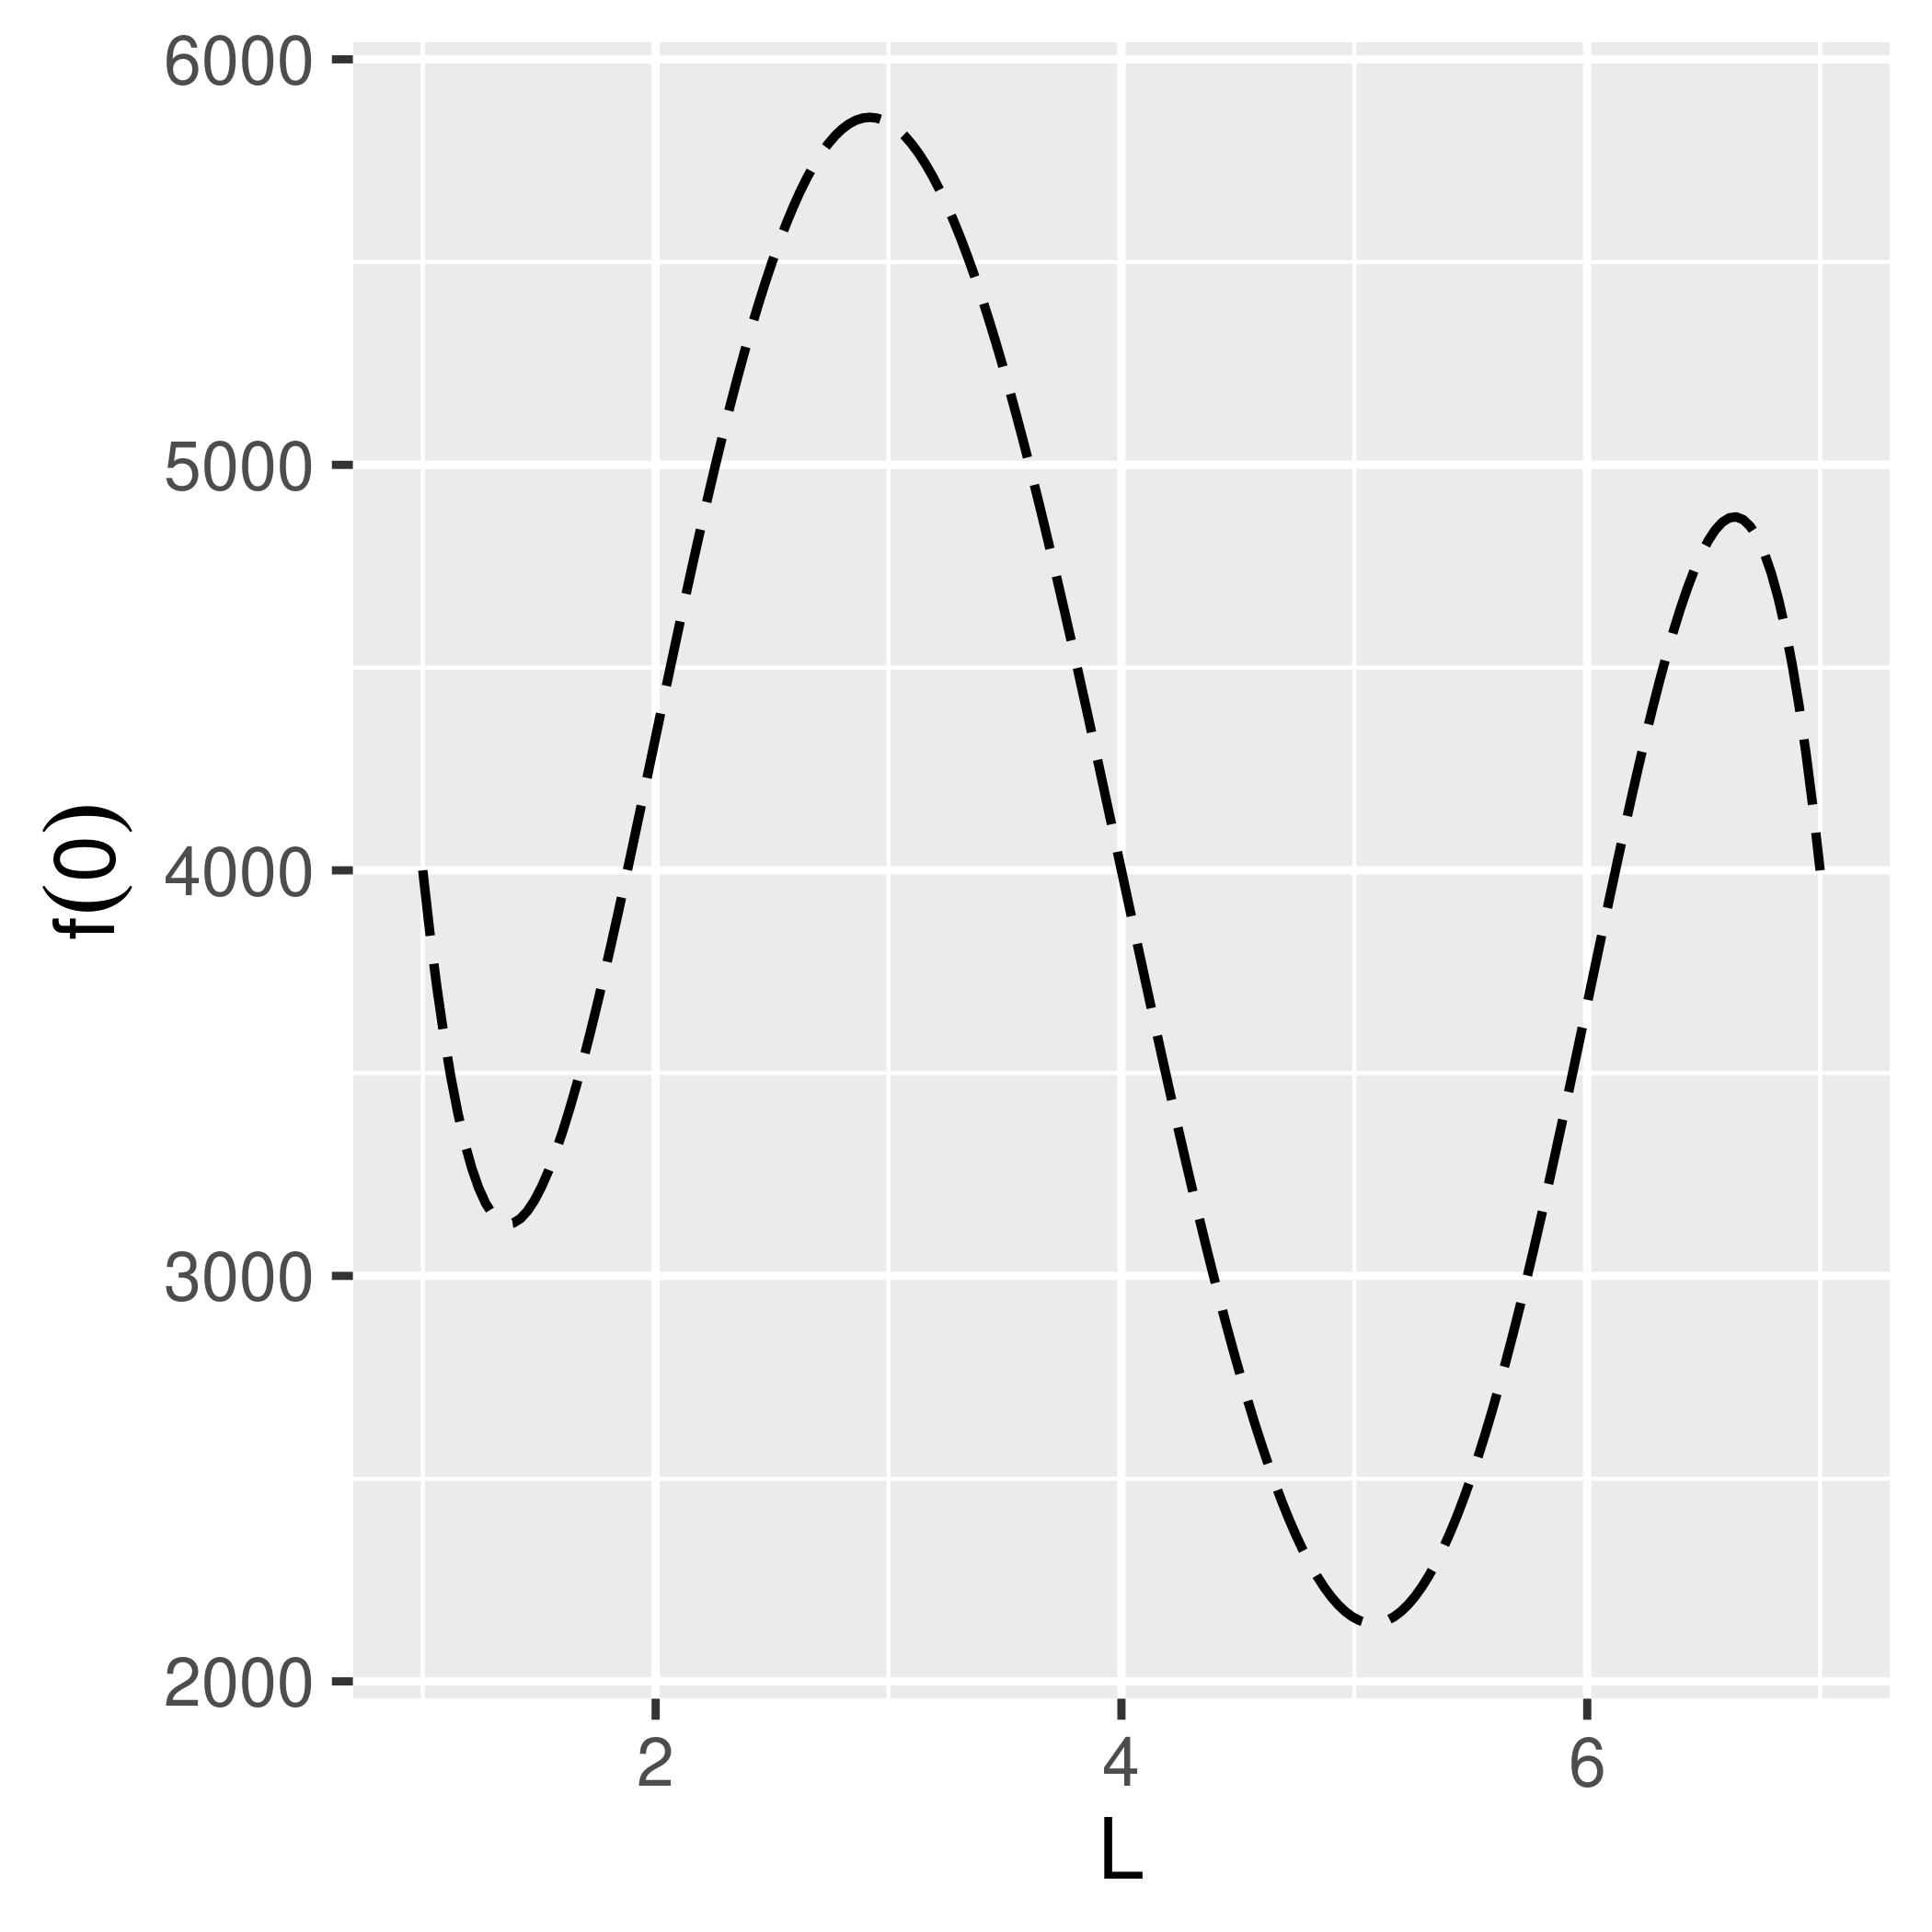
\includegraphics[width=0.6\textwidth]{initial_psd.png}
    \caption{ 
      Initial condition.
    }
    \label{fig:initialpsd}
  \end{subfigure}
  \hfill
  \begin{subfigure}[b]{0.75\textwidth}
    \centering
    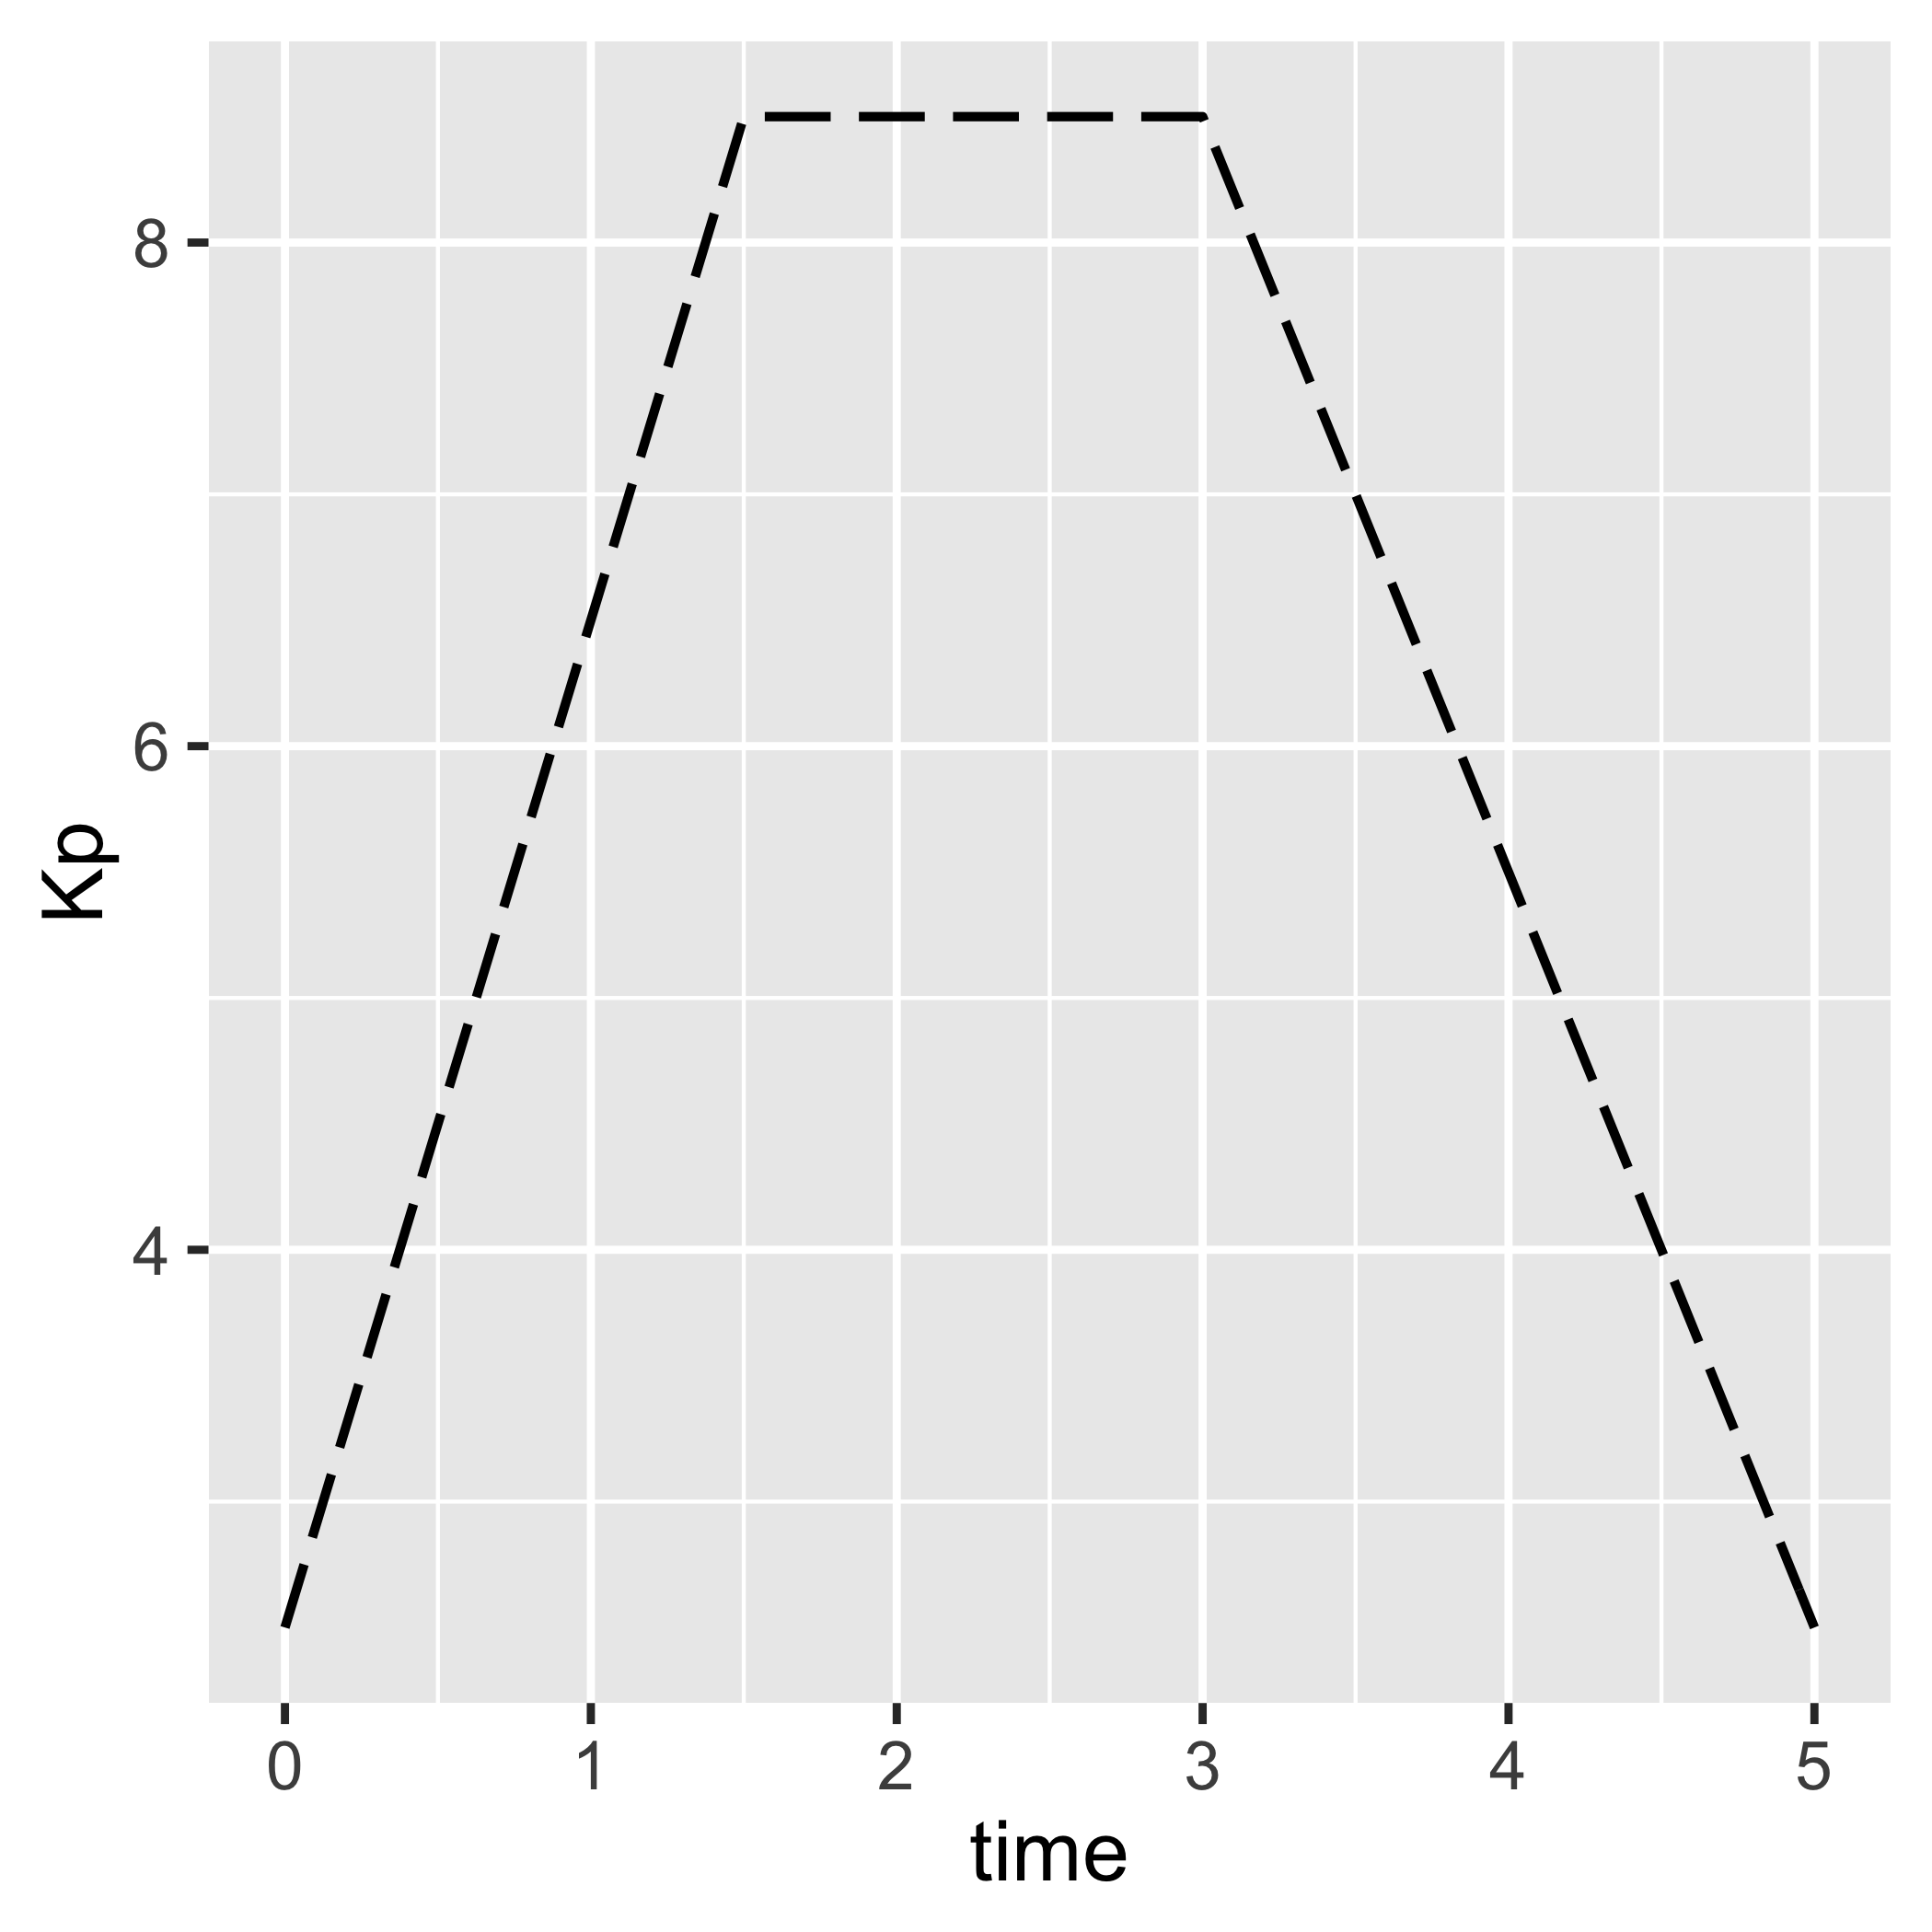
\includegraphics[width=0.6\textwidth]{kp_profile.png}
    \caption{
      Kp evolution.
    }
    \label{fig:kpProfile}
  \end{subfigure}
  \caption{Synthetic data generation for experiments.}
\end{figure*}

\subsubsection*{Data Generation}

\begin{table}[t]
  \caption{Parameters: Ground Truth}
  \label{tab:ground-truth}
  \centering
  \begin{tabular}{llll}
    \hline
    \textbf{Quantity}  & $\alpha$ & $\beta$ & $b$ \\
    \hline
    $q$ & $-1$  & $2.5$ & $0.75$  \\
    $\kappa$  & $\log(4.731 \times 10^{-10})$ & $10$ & $0.506$ \\
    $\lambda$ & $\log(0.3678)$ & $0.5$ & $-0.2$ \\
    \hline
  \end{tabular}
\end{table}

The technique presented is applied on synthetic data generated using a radial diffusion solver, 
the ground truth values of the radial diffusion parameters are listed in \cref{tab:ground-truth}.
%
The initial phase space density $f(t = 0)$ is set as follows (see \cref{fig:initialpsd}):
%
\begin{align*}
f(t = 0) &= 2000 + 500(C_{3}(\ell_*) - C_{5}(\ell_*)) \\
\ell_* &= 2\frac{\ell - \ell_{min}}{\ell_{max} - \ell_{min}} - 1 ,\\
\end{align*}
%
where $C_n(.)$ is the is the Chebyshev polynomial of degree $n$. The evolution of the Kp index is 
assumed to be an idealised version of a geomagnetic storm (see \cref{fig:kpProfile}) and 
defined as 
\[
  Kp(t) = \left\{\begin{matrix}
    2.5 & 0 \leq t < 2\\ 
    2.5 + 4(t - 2d) & 2 \leq t < 3.5\\ 
    8.5 & 3.5 \leq  t < 5 \\ 
    23.5 - 3t & 5 \leq t < 7\\
    2.5 & t \geq 7\\ 
    \end{matrix}\right. \ .
\] 
%
The radial diffusion solver is run for domain limits $\ell \in [1, 7], t \in [0, 9]$ with $200$ 
bins in the spatial and $50$ bins in the temporal domains respectively. After the approximate 
solution profiles of $f$ are generated, the points are sub-sampled uniformly such that $100$ points 
lying in the interior of the domain and $30$ points at the initial time step ($t = 0$) are 
selected. These observations are then perturbed by Gaussian noise to yield the final 
observation set $\mathcal{D}$ which is provided to the surrogate model $\hat{f}(x)$.


\begin{figure*}[!htb]
  \centering
  \begin{subfigure}[b]{0.5\textwidth}
    \centering
    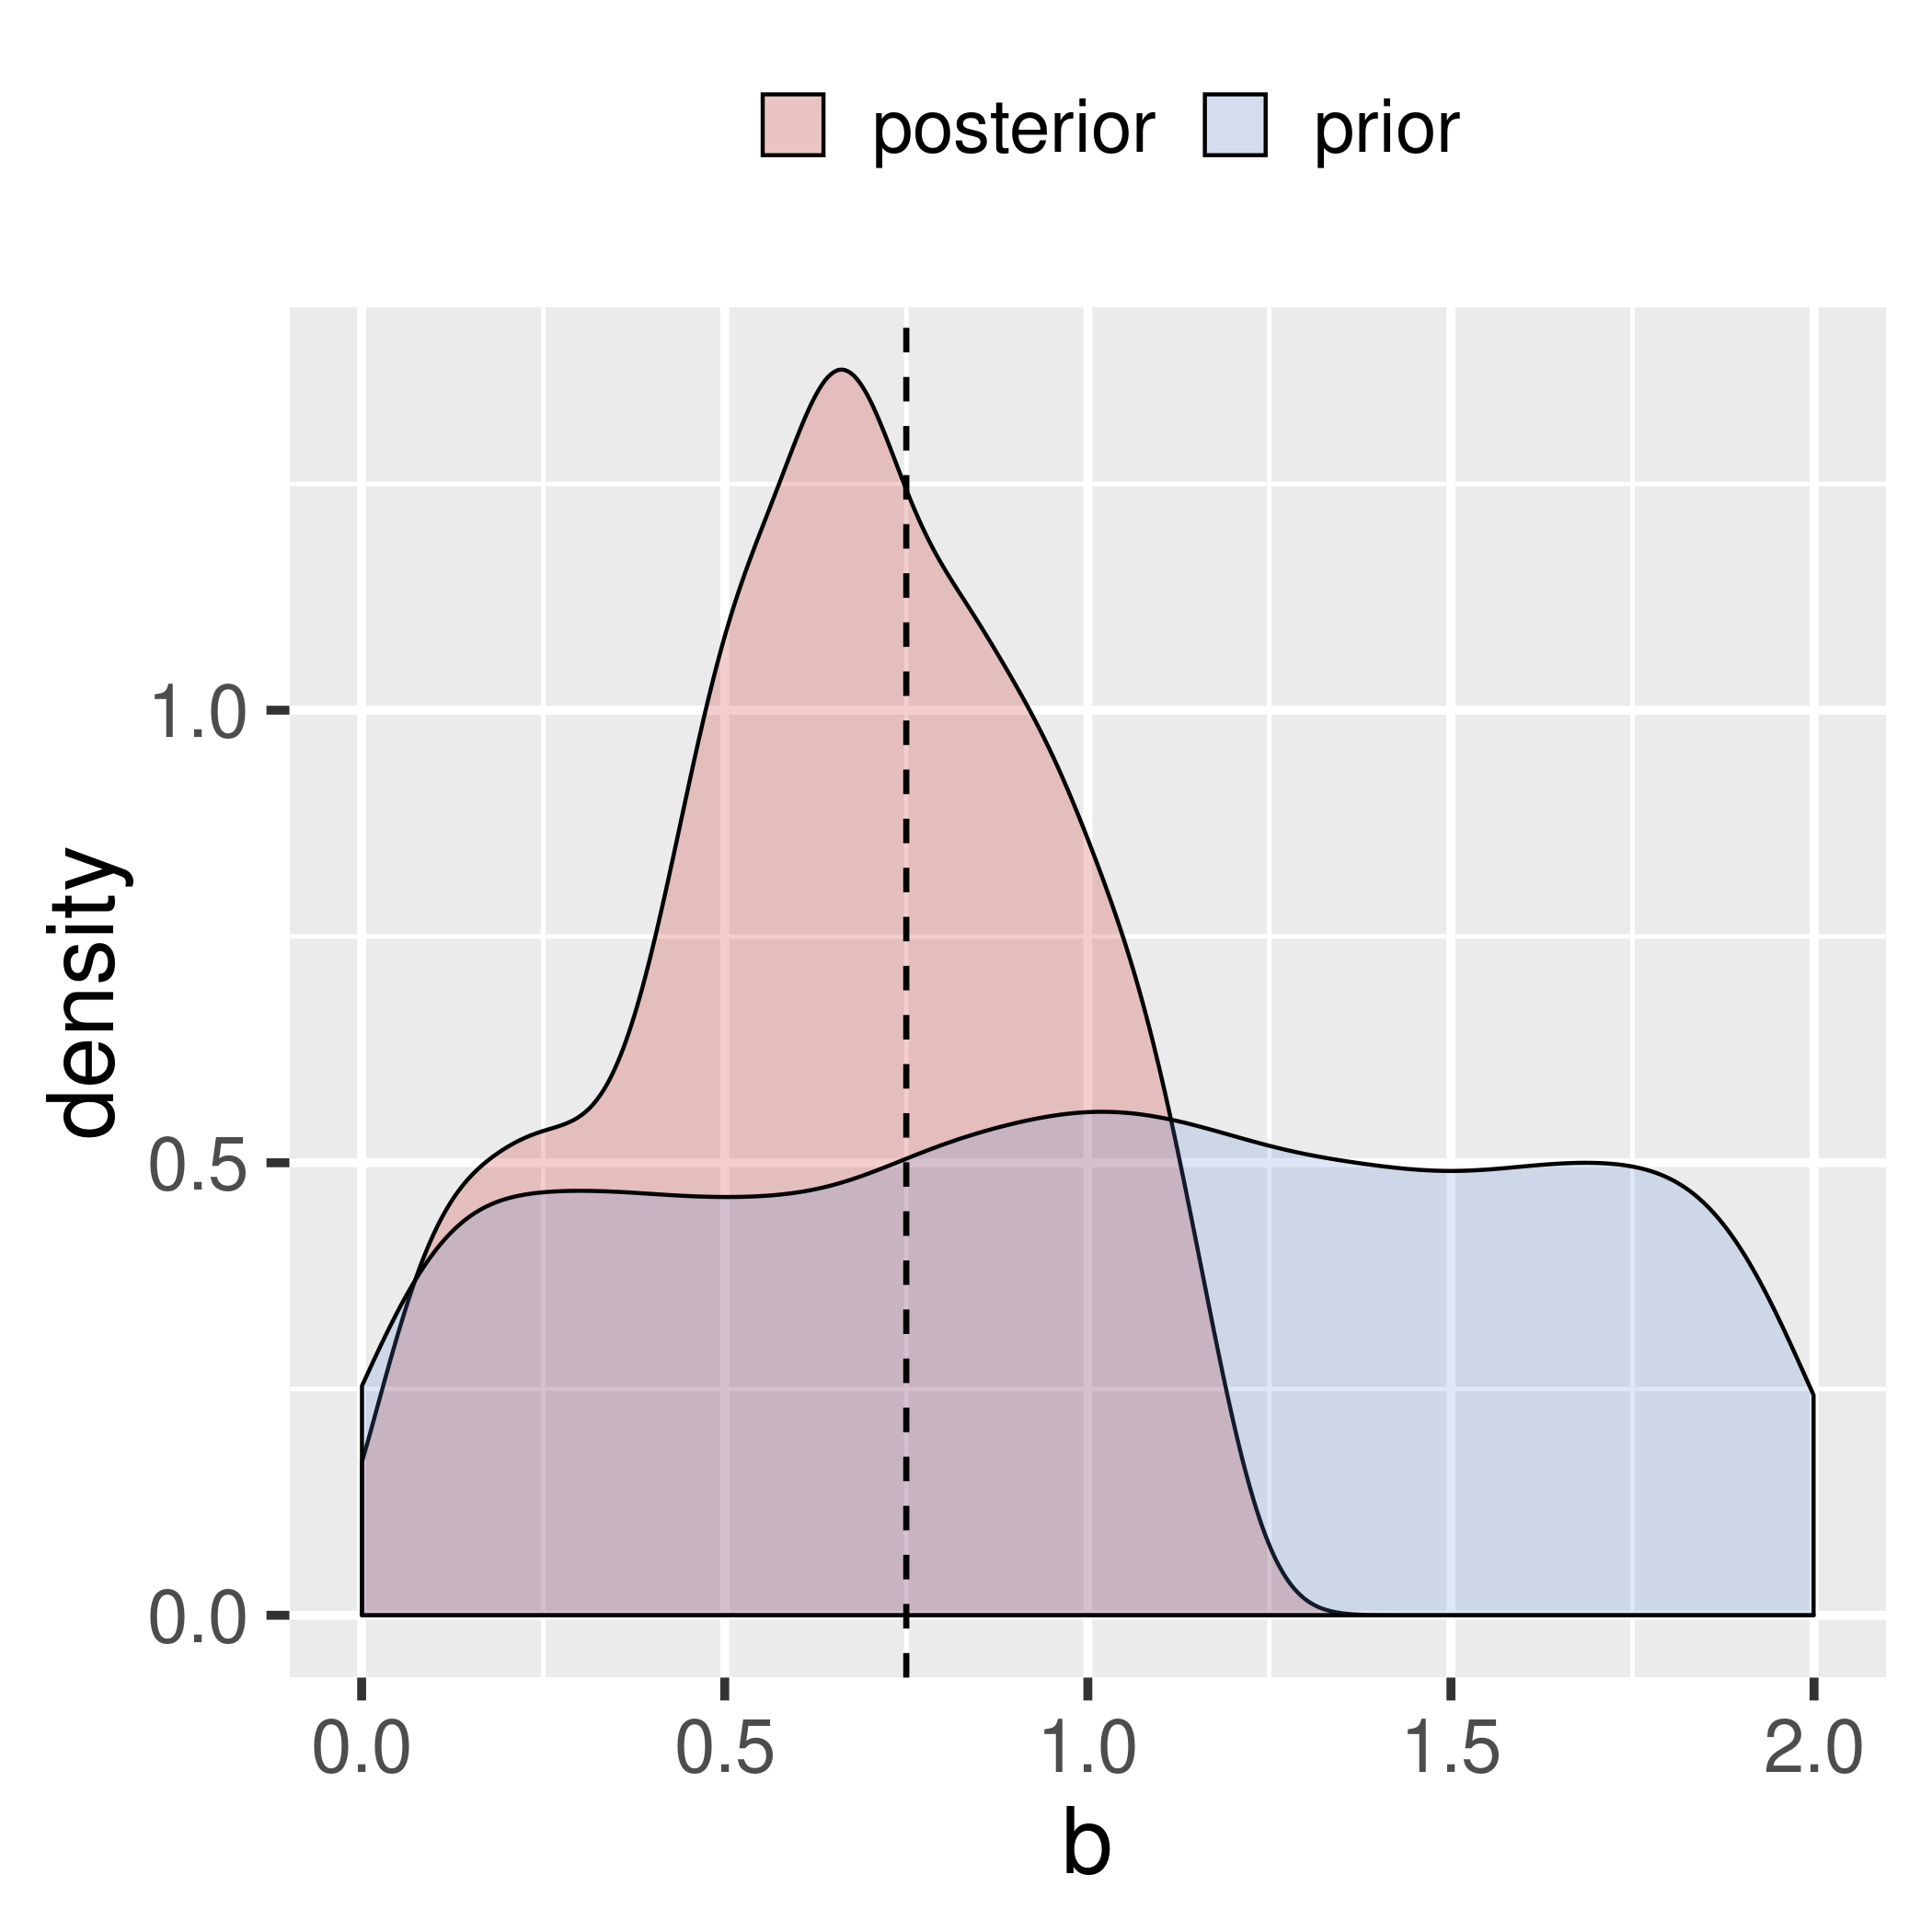
\includegraphics[width=0.6\textwidth]{density_Q_b.png}
    \caption{ Parameter $b$}
    \label{fig:qb}
  \end{subfigure}
  \hfill
  \begin{subfigure}[b]{0.5\textwidth}
    \centering
    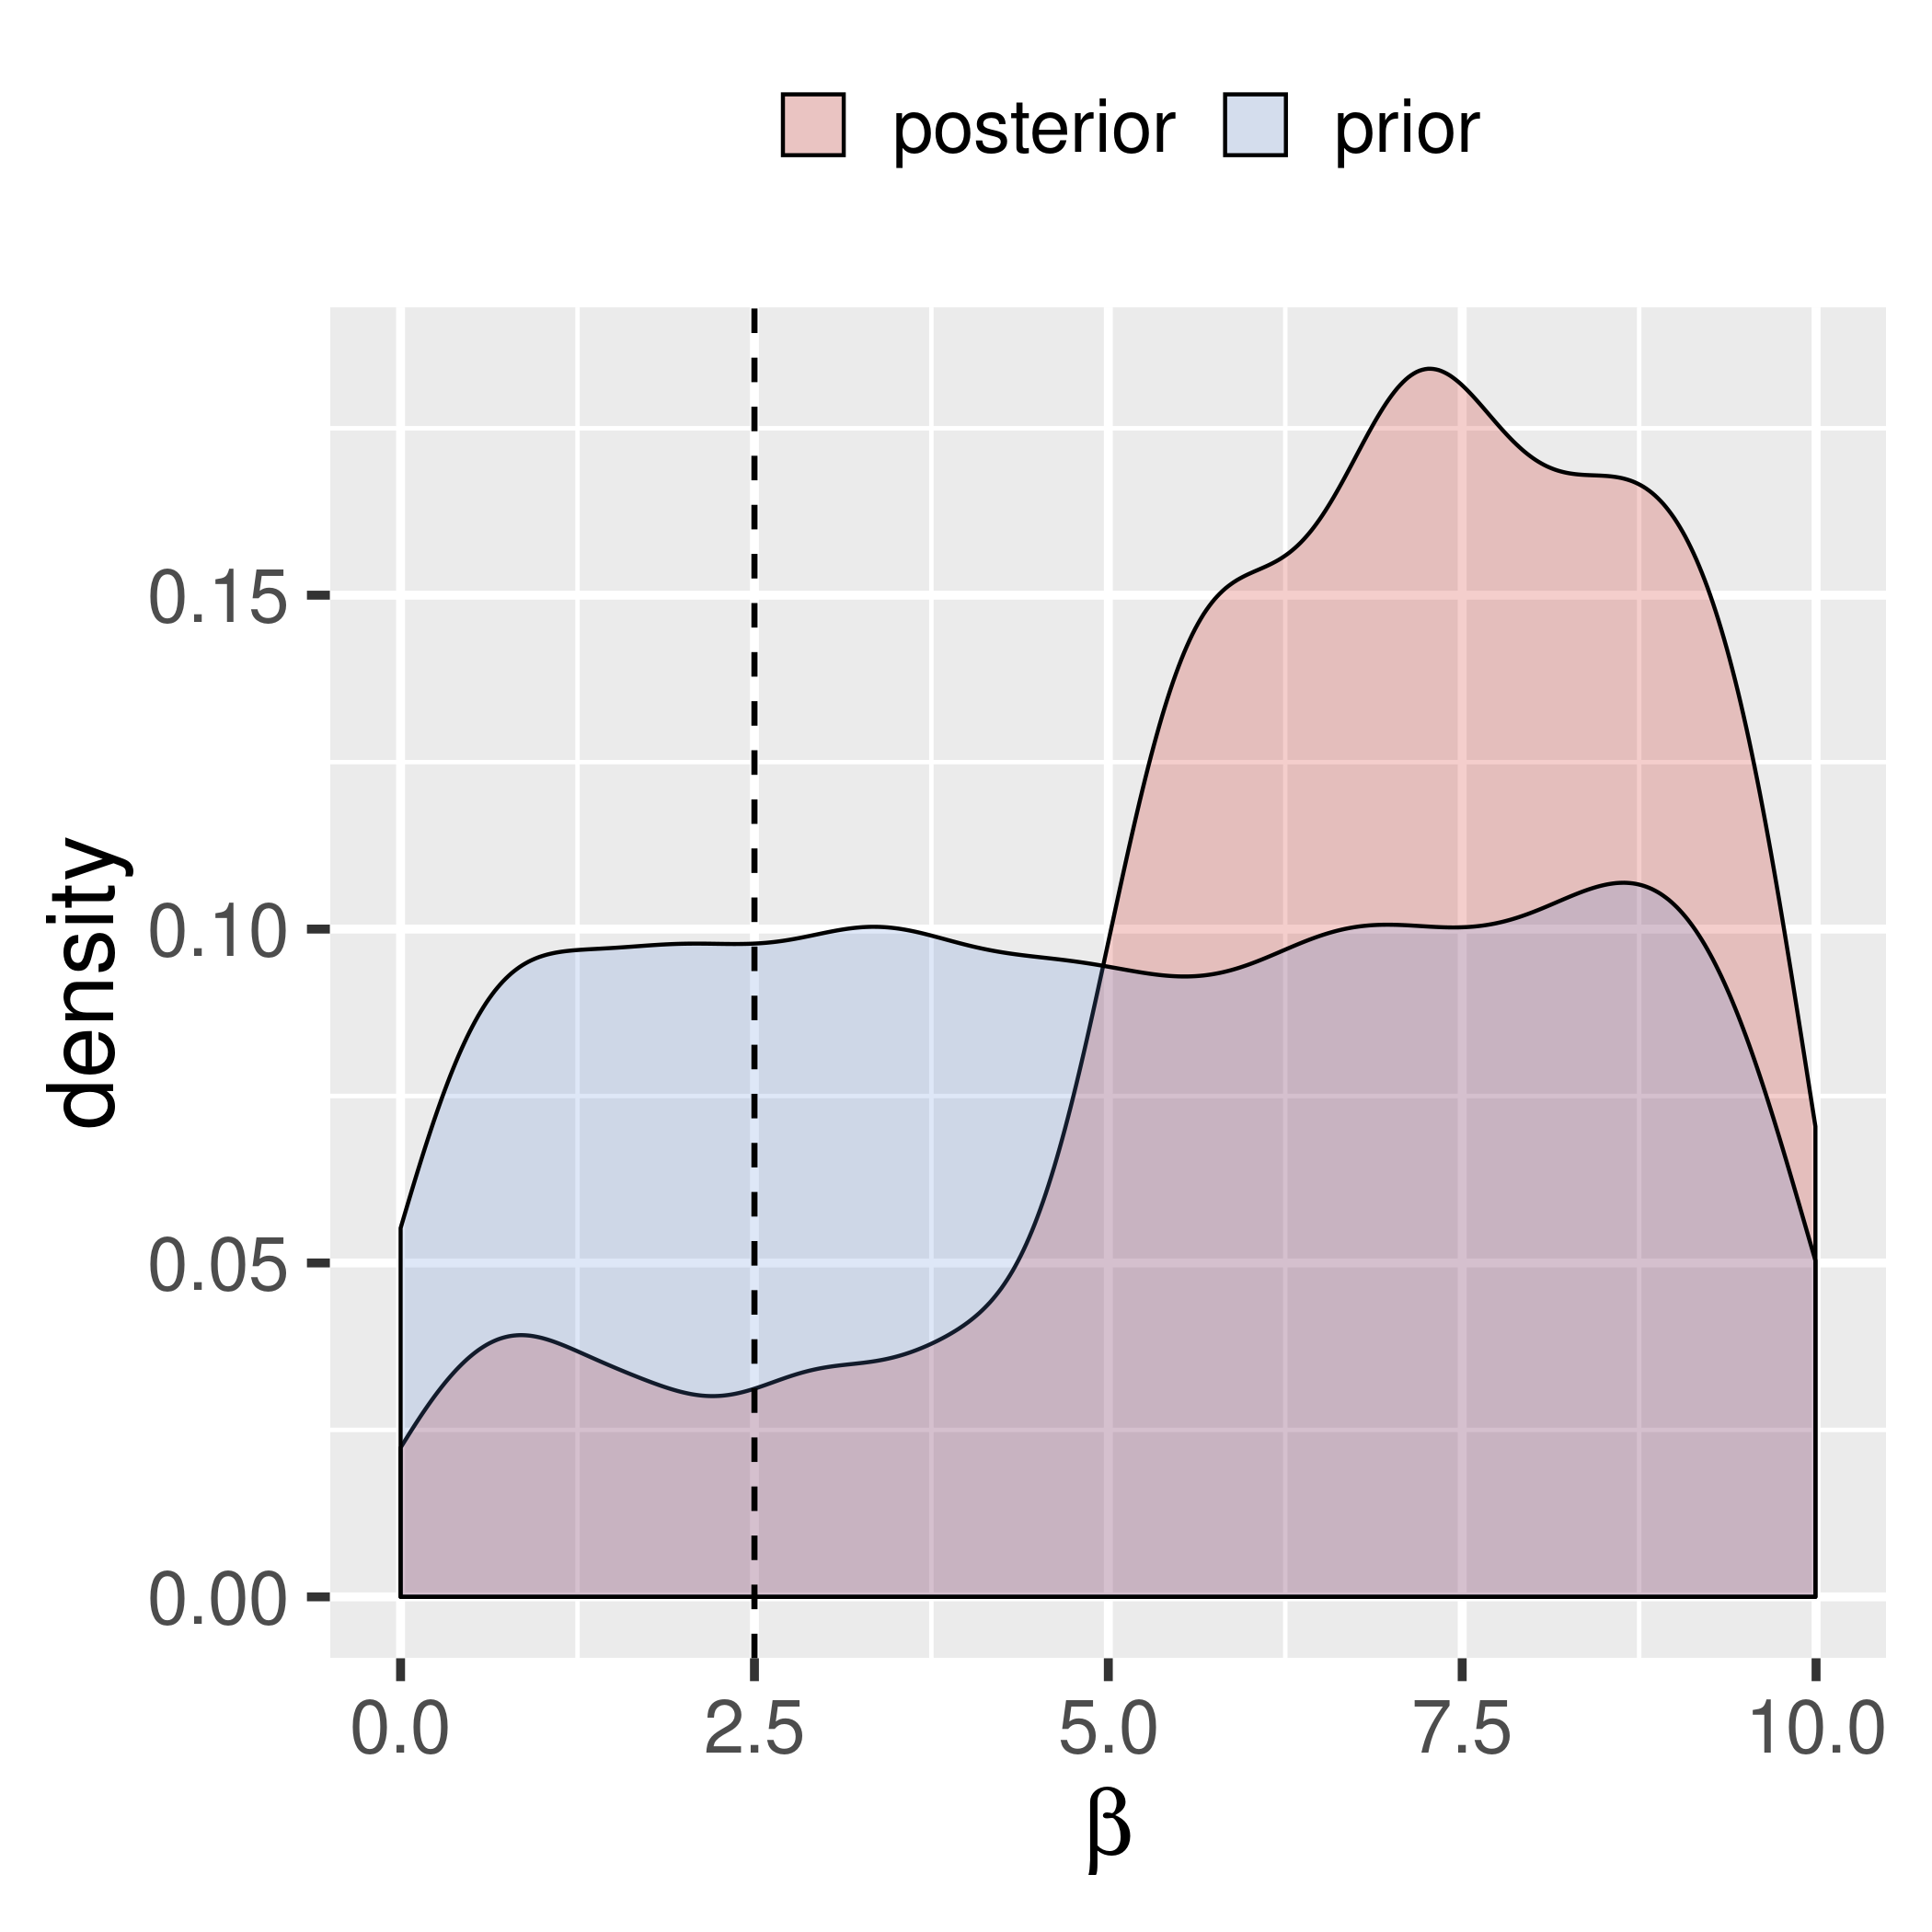
\includegraphics[width=0.6\textwidth]{density_Q_beta.png}
    \caption{Parameter $\beta$}
    \label{fig:qbeta}
  \end{subfigure}
  \hfill
  \begin{subfigure}[b]{0.5\textwidth}
    \centering
    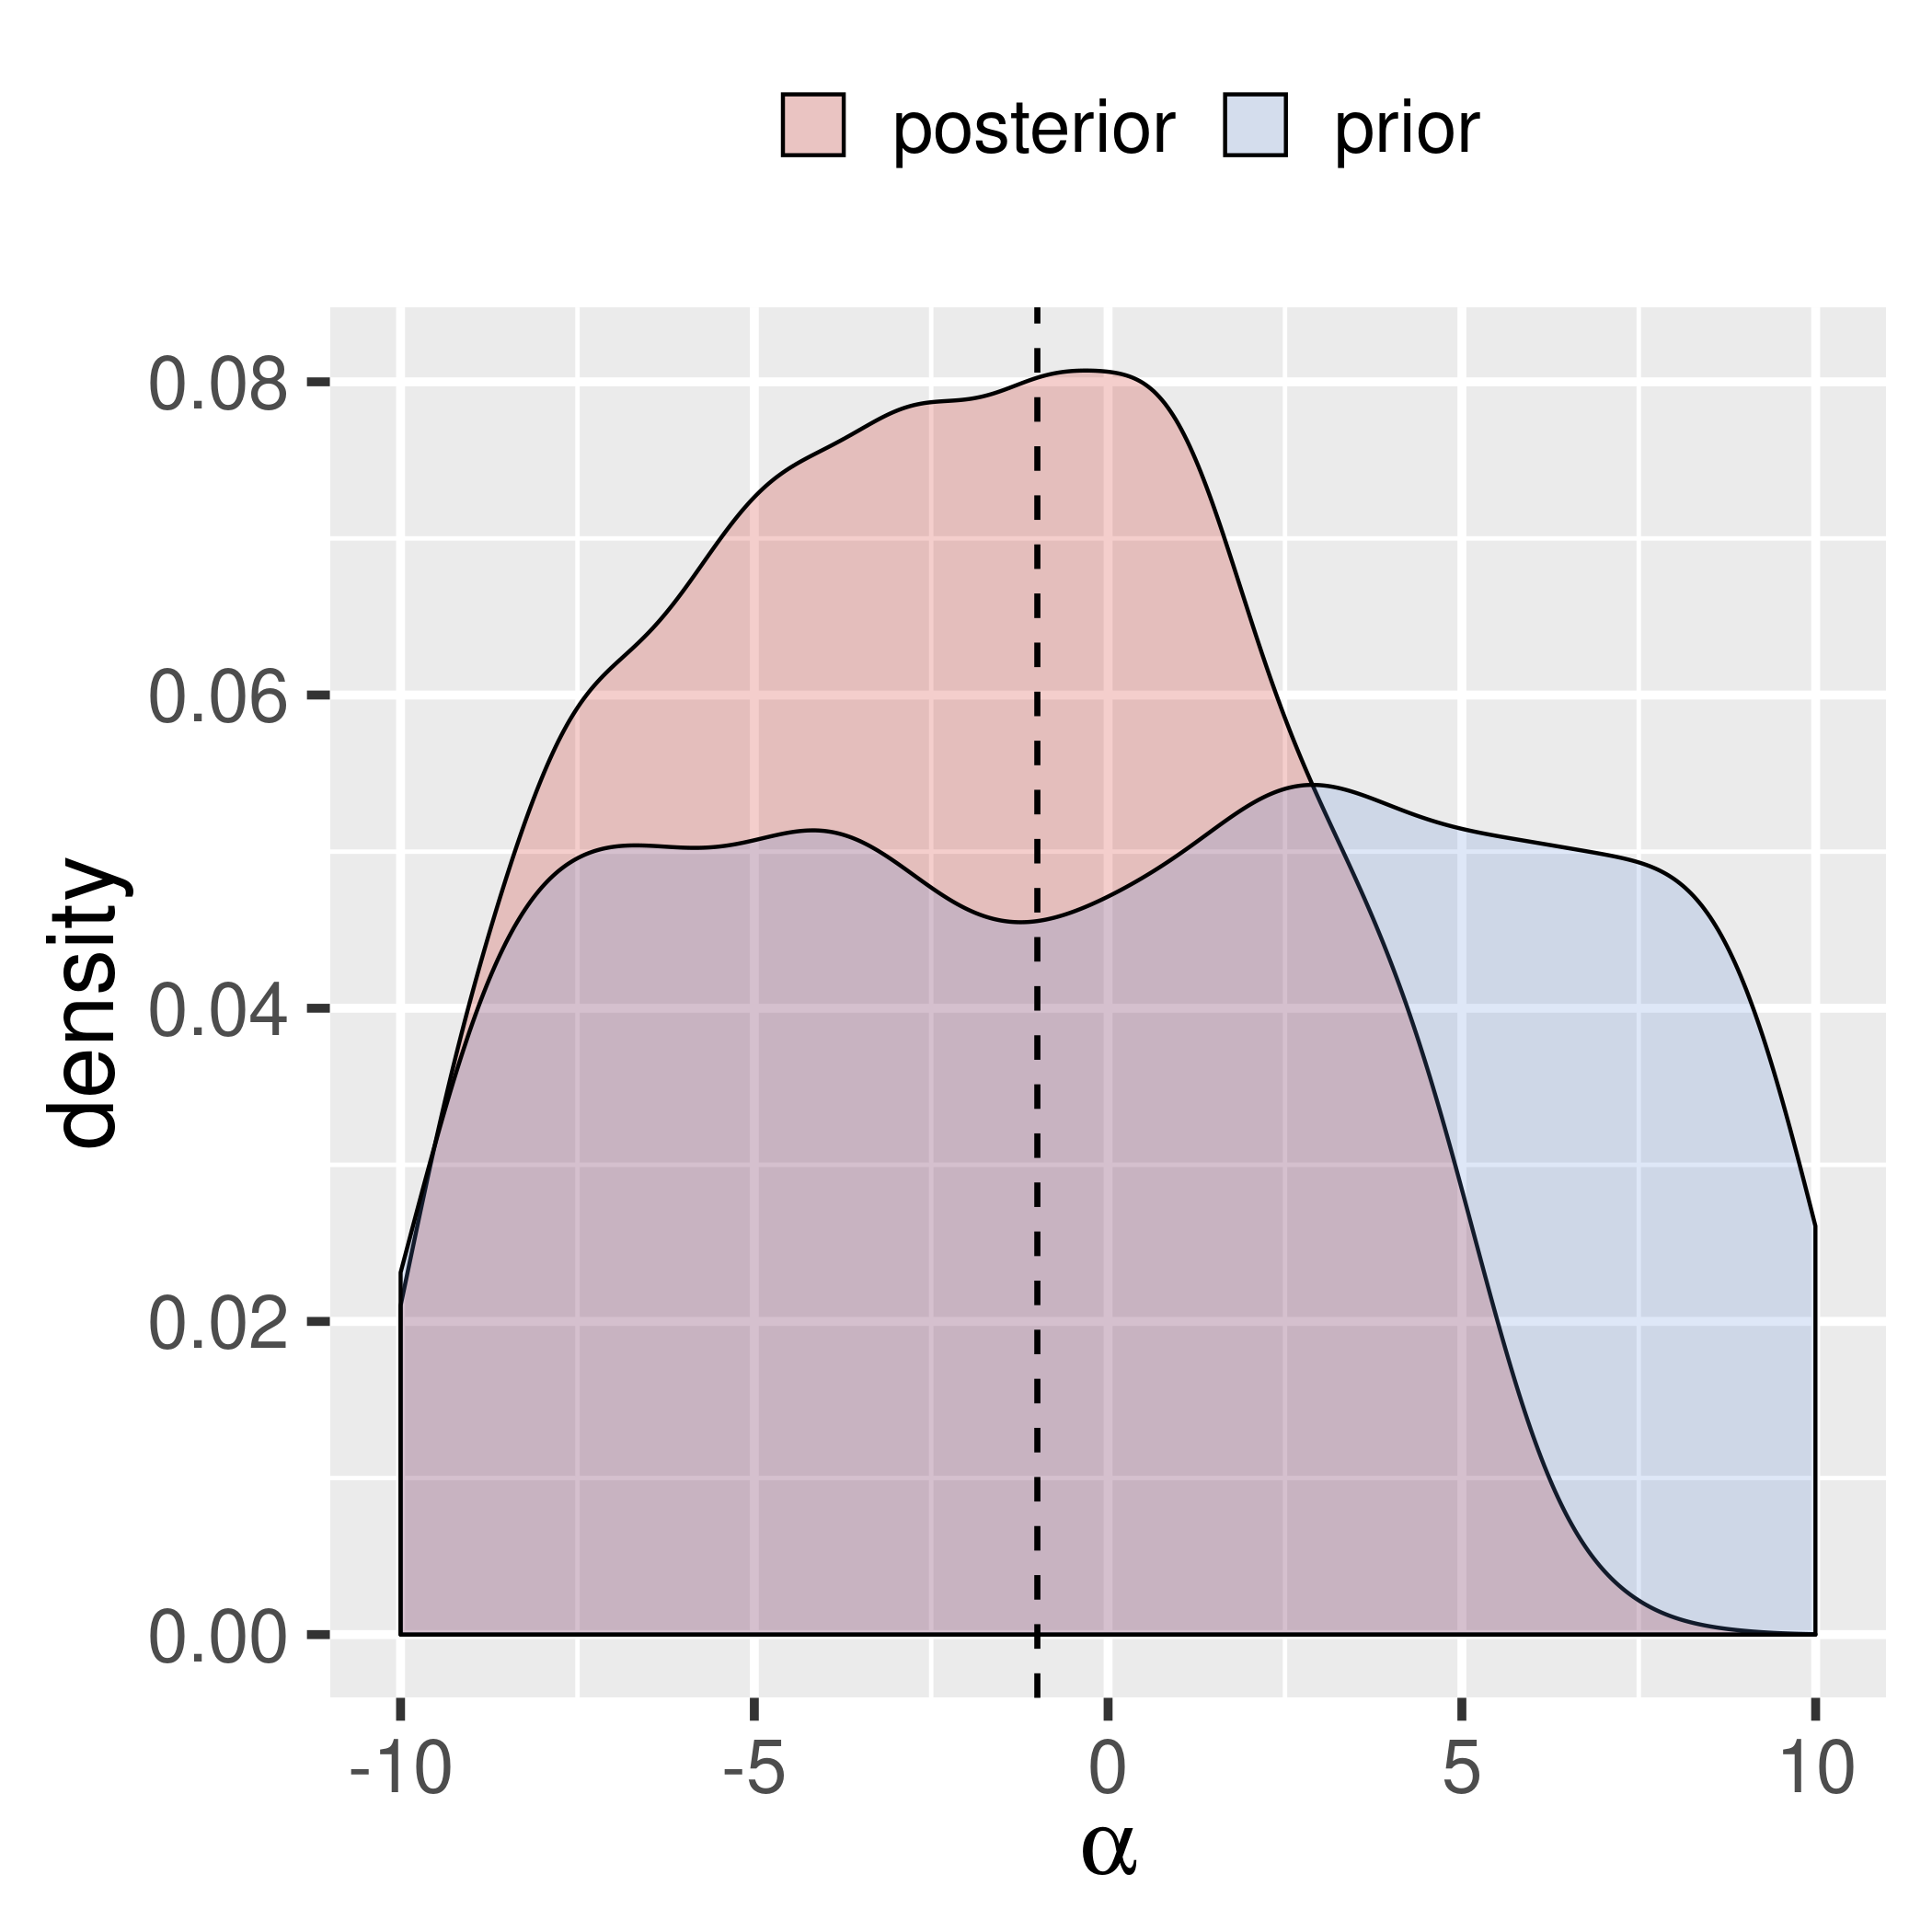
\includegraphics[width=0.6\textwidth]{density_Q_alpha.png}
    \caption{Parameter $\alpha$}
    \label{fig:qalpha}
  \end{subfigure}
  \caption{Comparing prior and posterior densities of the parameters of $q(\ell, t)$, 
  the black dotted line indicates the ground truth.}  
\end{figure*}


\section{Results}

The inferred posterior distribution for parameters of the particle injection rate $q(\ell, t)$ in 
\cref{fig:qalpha,fig:qbeta,fig:qb}. We see that the marginal posterior distributions of each 
parameter have high probability density near the ground truth, and that they are heavy tailed 
because there are often large regions of the parameter space which produce similar solutions for 
the phase space density $f$. Apart from identifying of parameters, the model also helps in 
significant reduction of uncertainty from prior to posterior for the parameters $\beta$, 
$\gamma$ and $b$.

The strength of the proposed method is the ability to quantify the uncertainty in diffusion 
parameters from a sparse set of observations. Due to the formulation of the surrogate as a dual 
optimization problem, it allows the inference to scale well with respect to high dimensional basis 
function expansions. The method shows promise for parameter inference of physical systems and 
warrants further research in its improvement.




\begin{figure*}[!htb]
  \centering
  \begin{subfigure}[b]{0.75\textwidth}
    \centering
    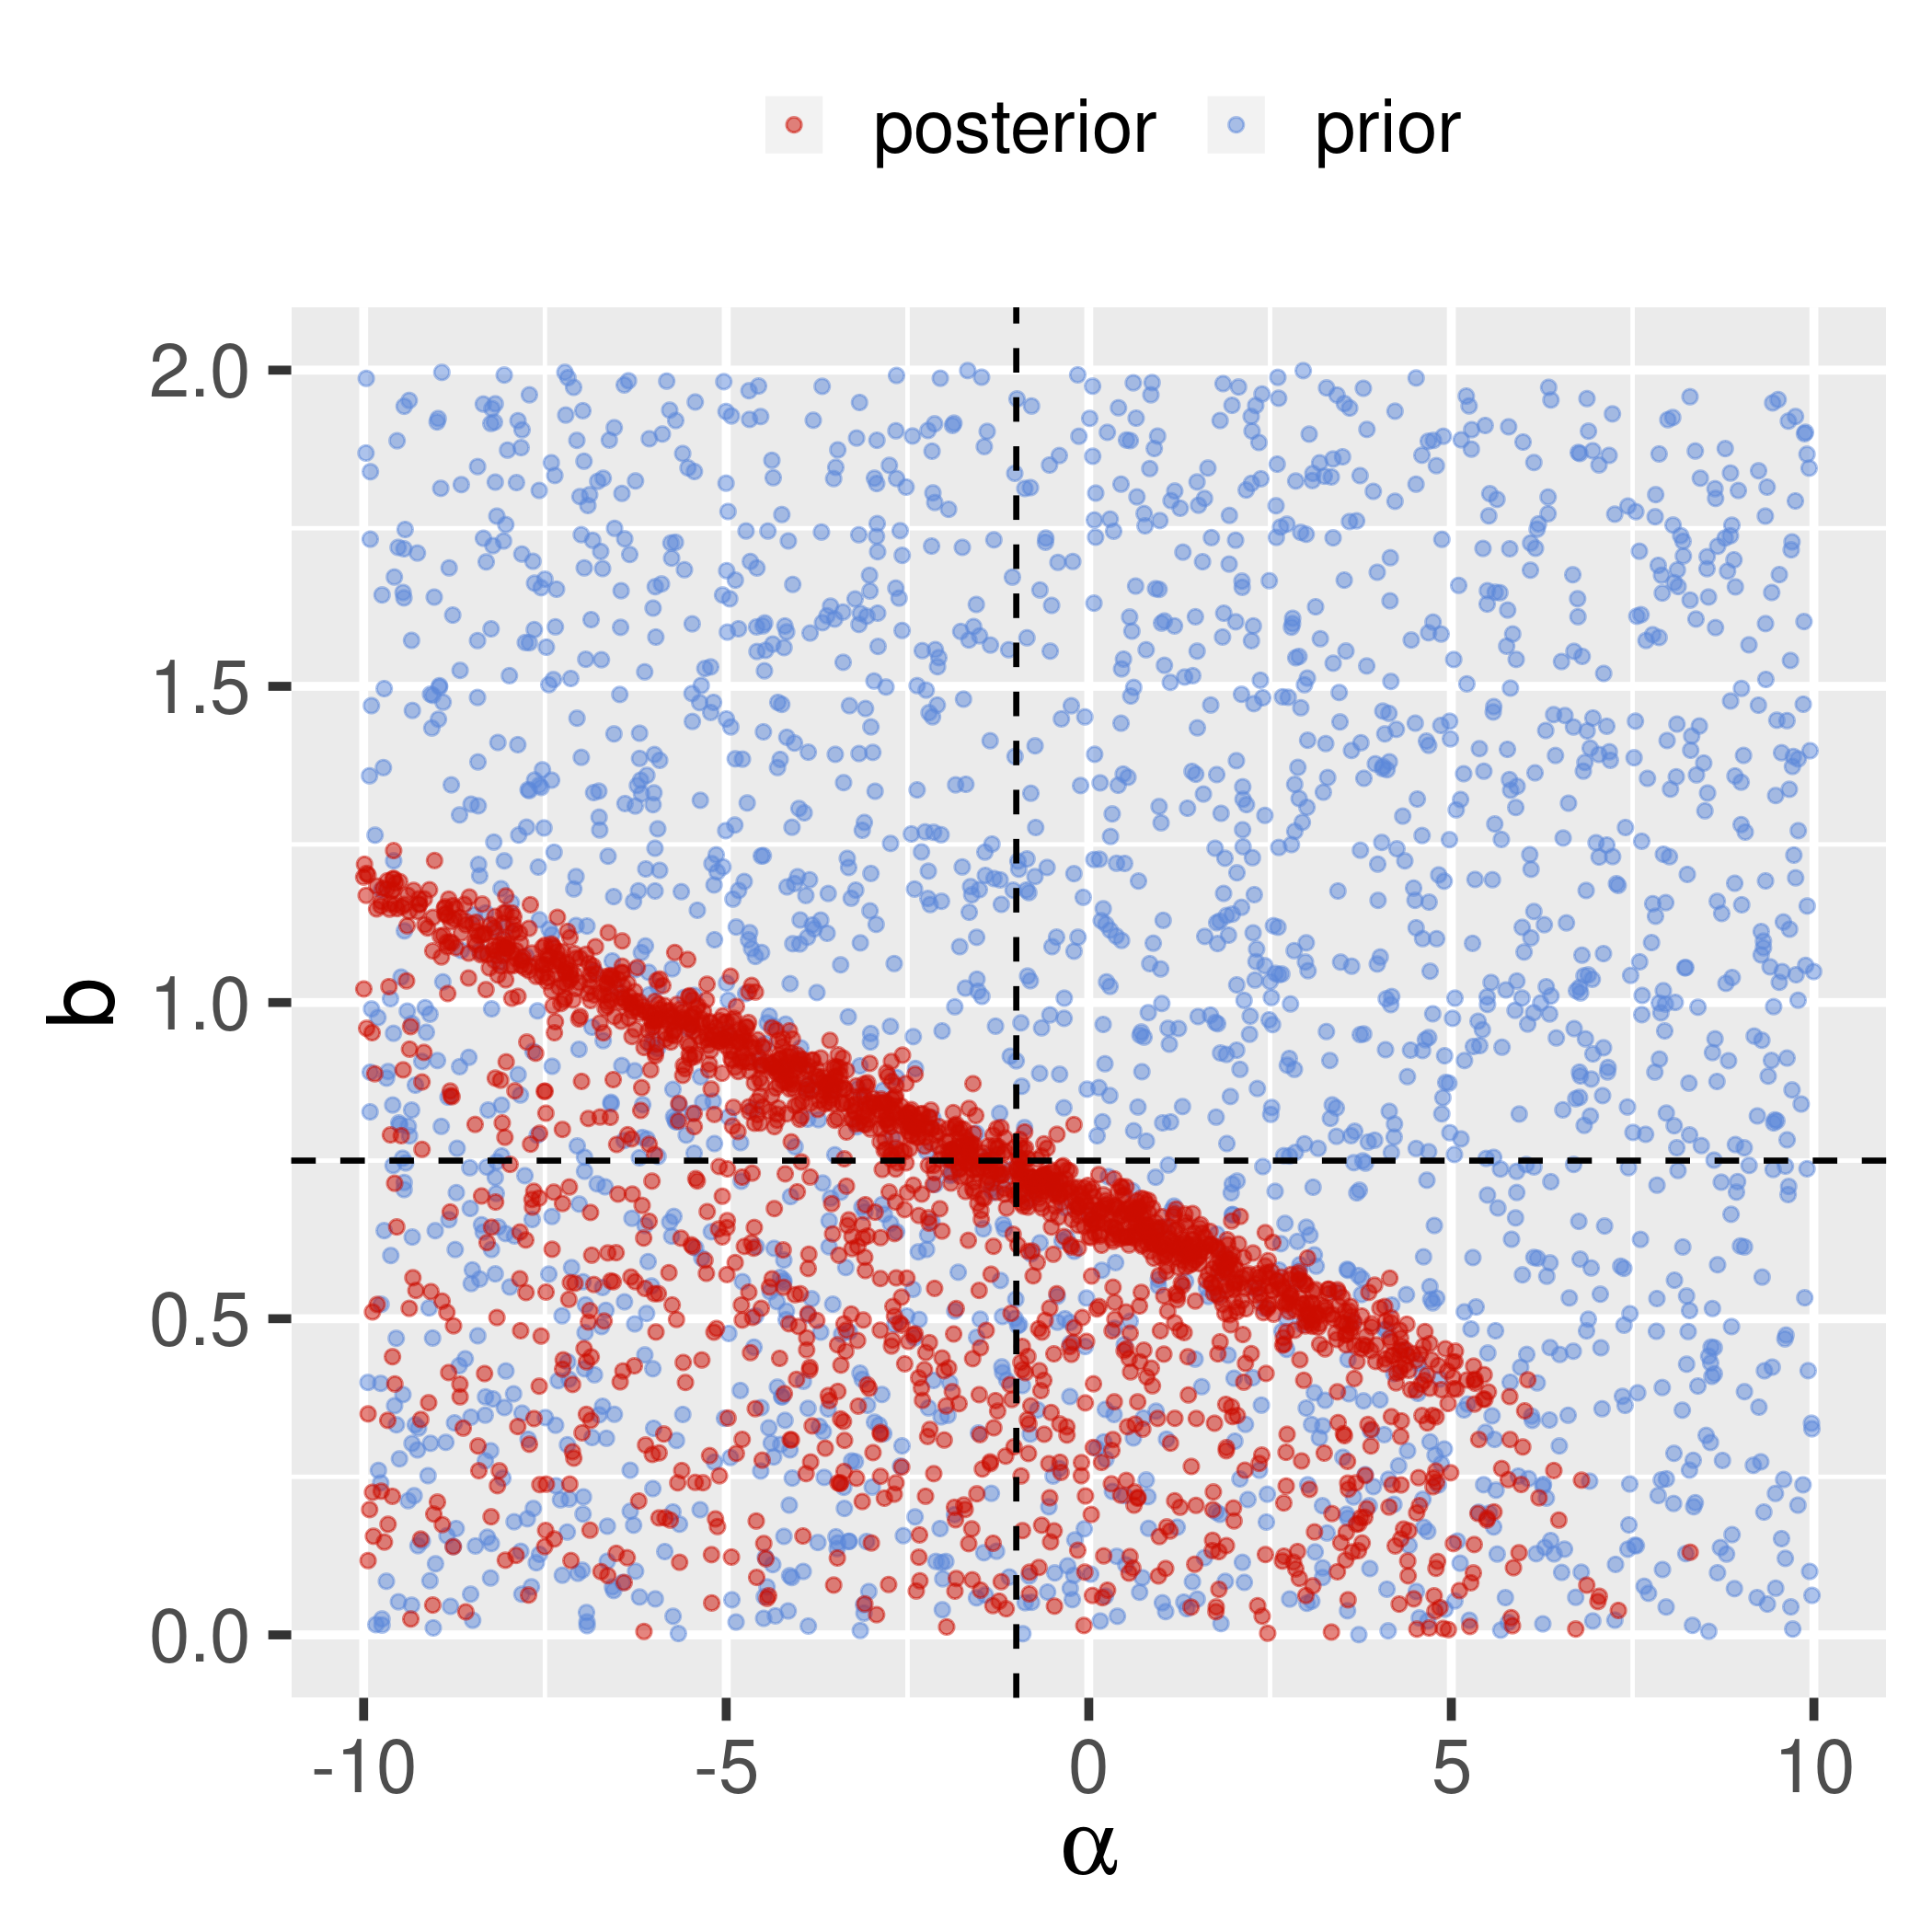
\includegraphics[width=0.6\textwidth]{prior_posterior_scatter_Q_alpha_b.png}
    \caption{ 
      Scatter chart: $\alpha$ versus $b$.  
    }
    \label{fig:alphavsb}
  \end{subfigure}
  \hfill
  \begin{subfigure}[b]{0.75\textwidth}
    \centering
    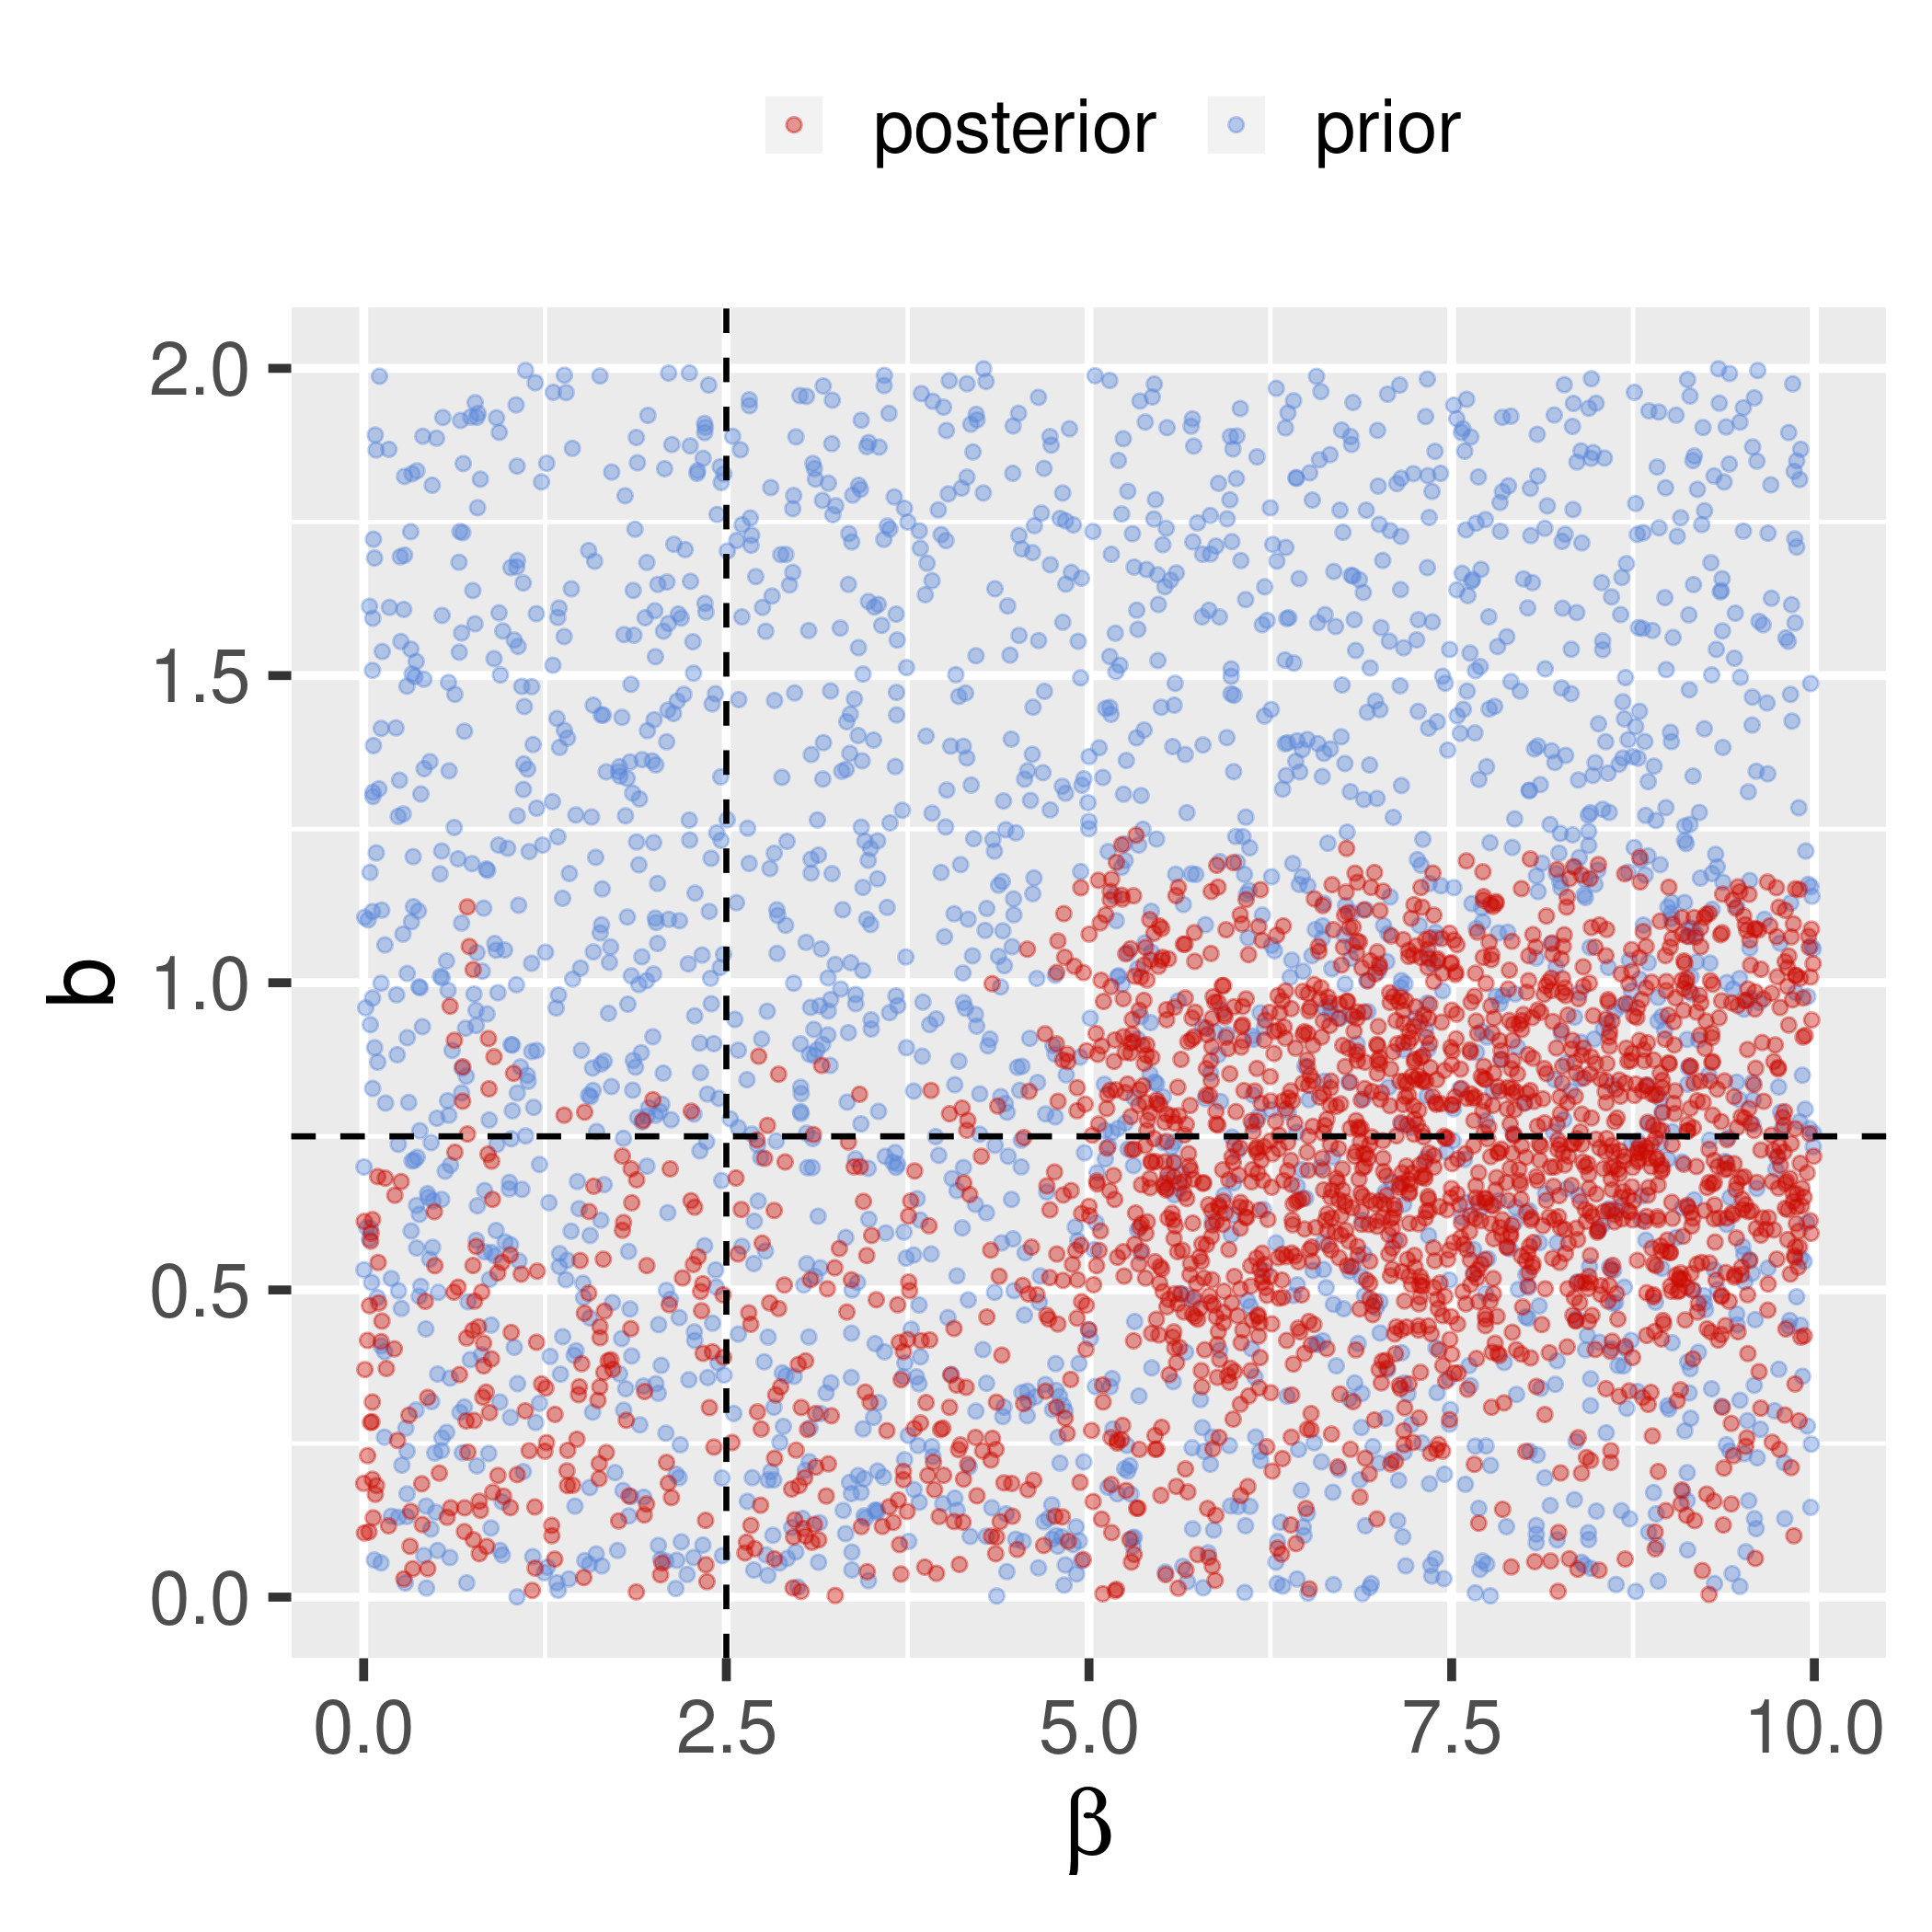
\includegraphics[width=0.6\textwidth]{prior_posterior_scatter_Q_beta_b.png}
    \caption{
      Scatter chart: $\beta$ versus $b$.  
    }
    \label{fig:betavsb}
  \end{subfigure}
  \caption{
    Comparing prior and posterior samples drawn from parameters of $q(\ell, t)$.
  }
\end{figure*}

%\bibliographystyle{plainnat}
%\bibliography{references}
